\documentclass[12pt,a4paper]{article}

\usepackage[a4paper,margin=1in]{geometry}
\usepackage{setspace}
\usepackage{graphicx}
\usepackage{booktabs}
\usepackage{longtable}
\usepackage{array}
\usepackage{amsmath,amssymb}
\usepackage{enumitem}
\usepackage{float}
\usepackage{xcolor}
\usepackage{hyperref}
\usepackage{caption}
\usepackage{subcaption}
\usepackage{fancyhdr}
\usepackage{titlesec}
\usepackage{tikz}
\usetikzlibrary{arrows.meta, positioning}

\onehalfspacing
\setlength{\parindent}{0pt}
\setlength{\parskip}{6pt}

\hypersetup{
    colorlinks=true,
    linkcolor=blue,
    citecolor=blue,
    urlcolor=blue
}

\pagestyle{fancy}
\fancyhf{}
\lhead{Explainable Generative AI-Based Financial Copilot}
\rhead{Research Report}
\cfoot{\thepage}

\titleformat{\section}{\Large\bfseries}{\thesection}{1em}{}
\titleformat{\subsection}{\large\bfseries}{\thesubsection}{1em}{}

\title{
\textbf{Explainable Generative AI-Based Financial Copilot}\\
for Personalized and Automated Financial Decision Support\\[0.5em]
\large Research Methodology, Simulation and Implementation Report
}

\author{
Saalini T\\
Department of Computing Technologies\\
SRM Institute of Science and Technology\\
Kattankulathur, Tamil Nadu, India
}

\date{\today}

\begin{document}

\maketitle

\begin{abstract}
Generative artificial intelligence has created new possibilities for financial decision-support systems that combine natural-language interaction, retrieval, personalization, reasoning, deterministic computation, and automated recommendations. However, a fluent recommendation is not necessarily correct, suitable for a particular user, or faithful to the actual factors that produced the decision. This research investigates an explainable generative-AI financial copilot for personalized household financial decision support. The proposed system is organized around five layers: generative substrate, grounding, personalization, reasoning and action, and explanation and governance. A central design principle is that explanations should be derived from inspectable decision artifacts---including retrieved evidence, user constraints, deterministic tool outputs, candidate decisions, and rejected alternatives---rather than treating a generated chain-of-thought-style rationale as proof of the decision process.

To support controlled experimentation, a synthetic household-finance benchmark has been constructed. The current simulation contains 1,000 synthetic financial profiles and 5,000 decision scenarios covering budgeting, debt prioritization, emergency-fund planning, investment allocation, and retirement planning. A deterministic ground-truth engine provides an independent reference decision for every scenario using bounded candidate catalogues, hard constraints, transparent scoring, deterministic ranking, and abstention. The benchmark has been validated for schema integrity, reproducibility, logical consistency, scenario integrity, and ground-truth determinism. At the time of this report, the Phase 6A experimental interfaces (a common input/output contract for four configurations) and the Phase 6B execution/orchestration layer are complete; the four configurations currently execute only clearly-labeled placeholder logic, with no language model, retrieval, or tool calls yet implemented. The subsequent experiments will compare a baseline LLM, a retrieval-augmented configuration, a personalized configuration, and the complete proposed financial copilot. This report documents the research motivation, literature findings, research gap, proposed solution, architecture, dataset design, simulation results, ground-truth methodology, experimental plan, implementation status, limitations, and reproducibility resources.
\end{abstract}

\textbf{Keywords:} Generative AI, Large Language Models, Financial Copilot, Explainable AI, Personalization, Retrieval-Augmented Generation, Financial Decision Support, Faithfulness, Abstention, AI Governance

\tableofcontents
\newpage

% =========================================================
\section{Introduction}

Financial decision-making is a high-consequence domain for artificial intelligence because an incorrect recommendation can directly affect an individual's savings, debt, investments, retirement plans, and financial stability. Traditional financial advisory services provide human expertise but can be expensive or inaccessible to some retail users. Robo-advisory systems have reduced some of these barriers, but they generally rely on structured questionnaires and relatively predefined investment recommendations.

Generative artificial intelligence changes this interaction model. Large language models can interpret natural-language questions, summarize financial information, maintain conversational context, retrieve information, reason over structured data, and invoke external tools. Financially specialized systems such as BloombergGPT and FinGPT have demonstrated the value of financial-domain adaptation, while agentic systems such as FinMem, FinRobot, and TradingAgents demonstrate how language models can be organized into structured financial workflows \cite{wu2023bloomberg,yang2023fingpt,yu2025finmem,yang2024finrobot,xiao2024tradingagents}.

These developments motivate the concept of a \textit{financial copilot}: a conversational and potentially agentic system that understands a user's financial context, retrieves relevant information, evaluates alternatives, and provides a recommendation or action.

However, financial decision support requires more than fluent generation. A system may produce a convincing explanation that does not faithfully represent the actual factors responsible for its recommendation. Classical explainability methods such as LIME and SHAP provide useful attribution mechanisms for structured predictive models, but they do not directly explain an entire generative workflow \cite{ribeiro2016lime,lundberg2017shap}. Research on generated rationales has further shown that readable reasoning is not necessarily faithful reasoning \cite{jacovi2020faithfulness,turpin2023unfaithful,lanham2023faithfulness}.

Therefore, this research focuses on building and evaluating a financial copilot whose decision process can be checked through explicit artifacts. The research does not treat the language model itself as the ground truth. Instead, a controlled synthetic benchmark and deterministic reference engine are constructed first, allowing later LLM configurations to be compared under identical conditions.

% =========================================================
\section{Background and Literature Review}

A literature review was conducted across generative AI for finance, financial language models, agent architectures, personalization, explainable AI, and responsible AI. The review covered work published between 2020 and 2026 and considered research from IEEE Xplore, ACM Digital Library, SpringerLink, ScienceDirect, and arXiv.

The review identified three broad research streams.

\subsection{Financial language models and agents}

BloombergGPT demonstrated the potential of large-scale financial-domain pretraining, while FinGPT emphasized an open and adaptable financial-language-model pipeline. Agentic systems such as FinMem, FinRobot, and TradingAgents demonstrated the use of memory, specialized roles, document analysis, and multi-agent workflows.

An important conclusion from the literature is that financial-domain language competence does not guarantee numerical correctness. Financial calculations such as loan amortization, compound growth, portfolio variance, and tax calculations are better delegated to deterministic tools.

\subsection{Personalization}

Traditional robo-advisory personalization commonly maps questionnaire responses to a risk profile or portfolio. More recent generative systems attempt to model richer user state, including income, assets, liabilities, spending, goals, risk tolerance, investment horizon, and persistent preferences.

The literature also shows that user satisfaction and emotional trust are not reliable proxies for advice quality. In particular, conversational style can increase perceived competence even when advice quality does not improve. Therefore, this research evaluates personalization using decision suitability, profile sensitivity, and preference/constraint handling rather than conversational satisfaction alone.

\subsection{Explainability and faithfulness}

Classical methods including LIME, SHAP, and counterfactual explanations remain valuable for structured sub-models. However, they do not directly solve the problem of explaining a stochastic generative workflow.

The literature distinguishes between a \textit{plausible explanation}, which sounds reasonable, and a \textit{faithful explanation}, which corresponds to the actual decision process. This distinction is central to the proposed system.

The literature review therefore adopts a hybrid explanation approach:
\begin{itemize}
    \item retrieved evidence provides checkable factual support;
    \item deterministic tool calls provide reproducible numerical evidence;
    \item constraint traces identify binding user requirements;
    \item candidate evaluation identifies rejected alternatives; and
    \item the final narrative communicates these artifacts to the user.
\end{itemize}

% =========================================================
\section{Research Gap}

The literature review identified five major gaps.

\subsection{G1: Explanation--Faithfulness Gap}

Current systems can generate explanations that are understandable but whose relationship to the actual decision computation is unverified. Existing financial XAI methods do not directly address faithfulness of an end-to-end generative financial copilot.

\subsection{G2: Outcome-Based Personalization Gap}

Personalization is frequently evaluated using user satisfaction, perceived trust, or interaction quality. These measures do not establish that a recommendation is suitable for the user's actual constraints and goals.

\subsection{G3: Lack of a Household Personal-Finance Benchmark}

Existing financial benchmarks such as FinQA, FinanceBench, and FinBen focus primarily on financial question answering, company filings, numerical reasoning, and institutional financial tasks \cite{chen2021finqa,islam2023financebench,xie2024finben}. There is no equivalent controlled benchmark centered on household decisions such as budgeting, debt prioritization, emergency-fund adequacy, investment allocation, and retirement planning.

\subsection{G4: Consumer-Facing Action Guardrails}

Much agentic financial research concentrates on market analysis and trading. Household financial decisions can be less frequent but potentially highly consequential and difficult to reverse. Explicit guardrails and abstention therefore require dedicated evaluation.

\subsection{G5: Private Personalization with Auditable Explanation}

A personalized financial system needs detailed information about a user, while an auditable system needs a record of the evidence and constraints used in its decision. This creates a privacy and auditability tension.

% =========================================================
\section{Problem Statement}

The research problem addressed in this work is:

\begin{quote}
\textbf{How can a generative-AI financial copilot provide personalized household financial decision support while maintaining correctness, explanation faithfulness, suitability, appropriate abstention, and auditable provenance?}
\end{quote}

The proposed research therefore does not aim merely to create a financial chatbot. It aims to experimentally evaluate whether architectural controls around a language model can improve the reliability and explainability of financial decision support.

% =========================================================
\section{Research Objectives}

The objectives of the research are:

\begin{enumerate}
    \item Design a layered architecture for explainable generative-AI financial decision support.
    \item Construct a controlled synthetic household-finance benchmark.
    \item Generate realistic financial profiles with meaningful relationships between financial variables.
    \item Generate household decision scenarios covering multiple categories of financial decision-making.
    \item Construct an independent deterministic ground-truth decision engine.
    \item Implement progressively richer LLM-based configurations.
    \item Evaluate recommendation correctness against the deterministic benchmark.
    \item Evaluate explanation faithfulness using perturbation-based tests.
    \item Evaluate personalization through suitability and profile-sensitivity tests.
    \item Evaluate abstention and auditability as first-class properties of the system.
\end{enumerate}

% =========================================================
\section{Proposed Architecture}

The proposed financial copilot follows a five-layer architecture.

\begin{enumerate}
    \item \textbf{L1 -- Generative Substrate:} general or finance-adapted foundation model.
    \item \textbf{L2 -- Grounding:} retrieval over financial documents and structured information, together with deterministic tools.
    \item \textbf{L3 -- Personalisation:} user goals, risk profile, constraints, financial state, and persistent context.
    \item \textbf{L4 -- Reasoning and Action:} candidate generation, planning, constraint enforcement, ranking, recommendation, and abstention.
    \item \textbf{L5 -- Explanation and Governance:} evidence presentation, constraint traces, tool traces, provenance, audit logs, and human oversight.
\end{enumerate}

\begin{figure}[H]
\centering
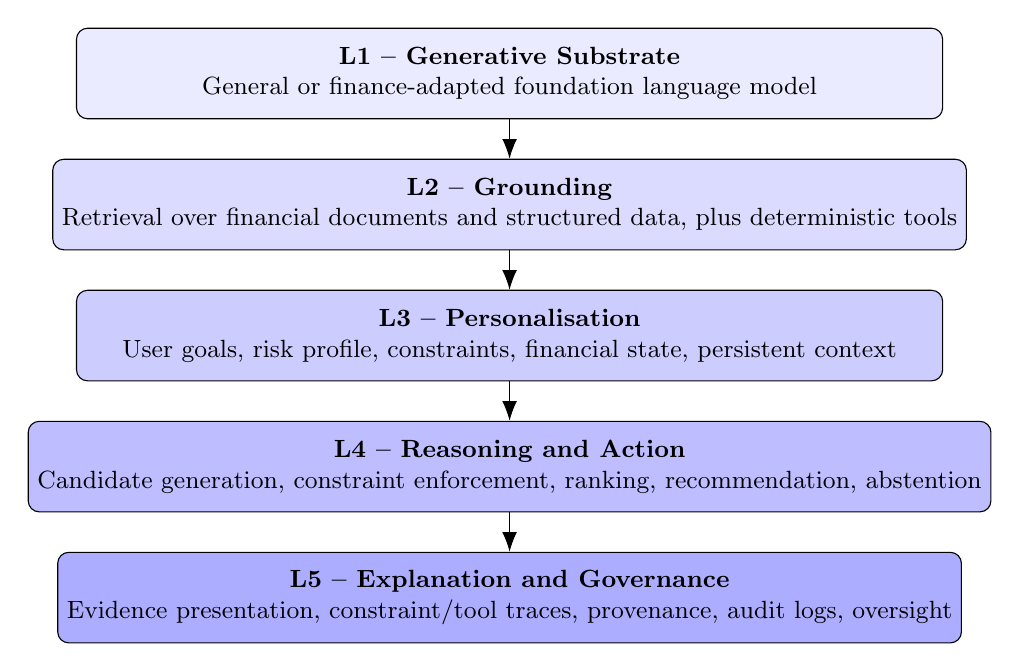
\begin{tikzpicture}[
    layer/.style={rectangle, draw, rounded corners, minimum width=11cm, minimum height=1.15cm, align=center, font=\small},
    node distance=0.5cm
]
\node[layer, fill=blue!8]              (l1) {\textbf{L1 -- Generative Substrate}\\ General or finance-adapted foundation language model};
\node[layer, fill=blue!14, below=of l1] (l2) {\textbf{L2 -- Grounding}\\ Retrieval over financial documents and structured data, plus deterministic tools};
\node[layer, fill=blue!20, below=of l2] (l3) {\textbf{L3 -- Personalisation}\\ User goals, risk profile, constraints, financial state, persistent context};
\node[layer, fill=blue!26, below=of l3] (l4) {\textbf{L4 -- Reasoning and Action}\\ Candidate generation, constraint enforcement, ranking, recommendation, abstention};
\node[layer, fill=blue!32, below=of l4] (l5) {\textbf{L5 -- Explanation and Governance}\\ Evidence presentation, constraint/tool traces, provenance, audit logs, oversight};

\draw[-{Latex[length=2.5mm]}] (l1) -- (l2);
\draw[-{Latex[length=2.5mm]}] (l2) -- (l3);
\draw[-{Latex[length=2.5mm]}] (l3) -- (l4);
\draw[-{Latex[length=2.5mm]}] (l4) -- (l5);
\end{tikzpicture}
\caption{Proposed five-layer architecture of the explainable financial copilot.}
\label{fig:architecture}
\end{figure}

The key design principle is that L5 should not simply ask the language model to describe its own hidden reasoning. Instead, the explanation should be assembled from artifacts produced by lower layers.

For example, a recommendation may be supported by:
\begin{itemize}
    \item the retrieved evidence used by the system;
    \item the user's binding constraints;
    \item the output of a loan or investment calculation tool;
    \item candidates considered and rejected; and
    \item the final deterministic ranking or confidence information.
\end{itemize}

% =========================================================
\section{Overall Research Workflow}

The research workflow separates benchmark generation, reference-decision construction, system implementation, and evaluation.

\begin{figure}[H]
\centering
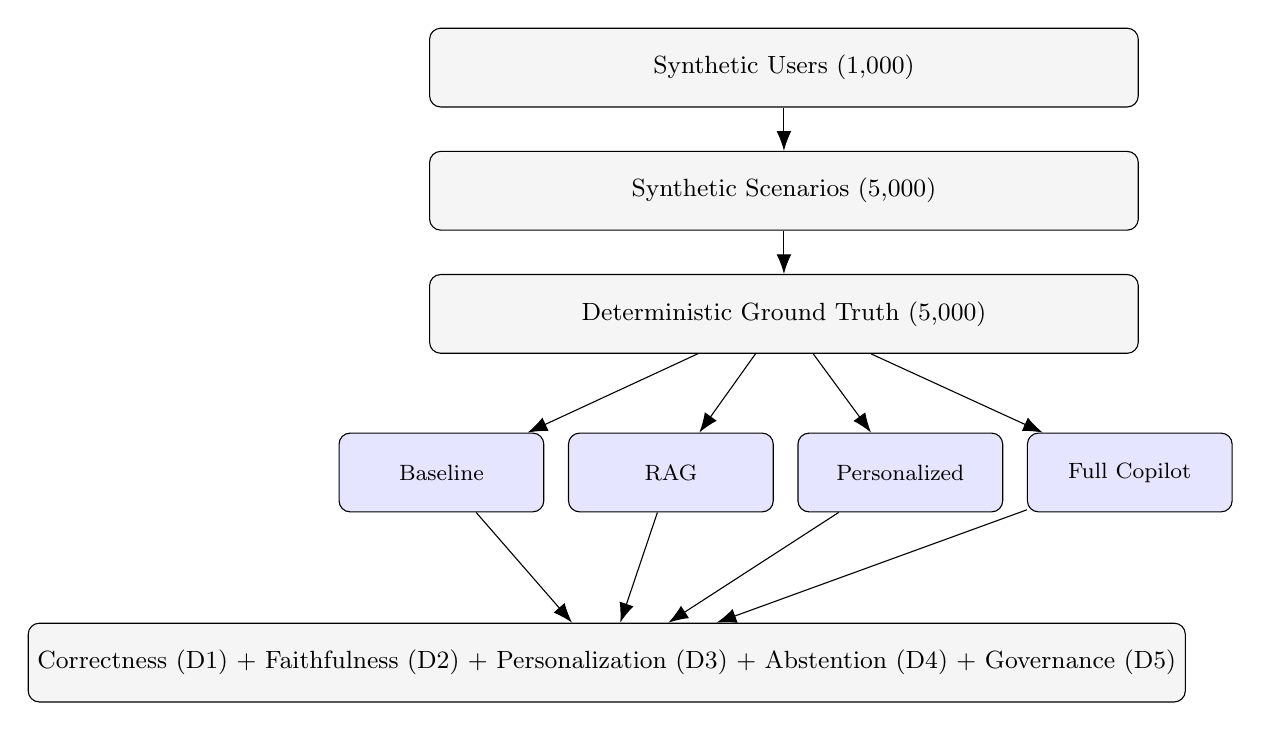
\begin{tikzpicture}[
    stage/.style={rectangle, draw, rounded corners, minimum width=9cm, minimum height=1cm, align=center, font=\small, fill=gray!8},
    cfgbox/.style={rectangle, draw, rounded corners, minimum width=2.6cm, minimum height=1cm, align=center, font=\footnotesize, fill=blue!10},
    node distance=0.55cm
]
\node[stage] (users) {Synthetic Users (1{,}000)};
\node[stage, below=of users] (scen) {Synthetic Scenarios (5{,}000)};
\node[stage, below=of scen] (gt) {Deterministic Ground Truth (5{,}000)};

\node[cfgbox, below=1.0cm of gt, xshift=-4.35cm] (base) {Baseline};
\node[cfgbox, right=0.3cm of base] (rag) {RAG};
\node[cfgbox, right=0.3cm of rag] (pers) {Personalized};
\node[cfgbox, right=0.3cm of pers] (full) {Full Copilot};

\node[stage, below=1.4cm of base, xshift=2.1cm] (metrics) {Correctness (D1) + Faithfulness (D2) + Personalization (D3) + Abstention (D4) + Governance (D5)};

\draw[-{Latex[length=2.5mm]}] (users) -- (scen);
\draw[-{Latex[length=2.5mm]}] (scen) -- (gt);
\draw[-{Latex[length=2.5mm]}] (gt) -- (base);
\draw[-{Latex[length=2.5mm]}] (gt) -- (rag);
\draw[-{Latex[length=2.5mm]}] (gt) -- (pers);
\draw[-{Latex[length=2.5mm]}] (gt) -- (full);
\draw[-{Latex[length=2.5mm]}] (base) -- (metrics);
\draw[-{Latex[length=2.5mm]}] (rag) -- (metrics);
\draw[-{Latex[length=2.5mm]}] (pers) -- (metrics);
\draw[-{Latex[length=2.5mm]}] (full) -- (metrics);
\end{tikzpicture}
\caption{End-to-end research and experimentation workflow.}
\label{fig:workflow}
\end{figure}

The important methodological property is that all experimental configurations use the same benchmark. This prevents differences in scenario difficulty or user population from becoming confounding variables.

% =========================================================
\section{Synthetic Dataset}

\subsection{Why a synthetic dataset is used}

No external real-world household financial dataset has been used for the current simulation. This is intentional.

A real financial dataset would introduce several problems:
\begin{itemize}
    \item privacy and personally identifiable financial information;
    \item incomplete or inconsistent household financial records;
    \item difficulty obtaining reliable ground-truth recommendations;
    \item inability to deliberately construct edge cases; and
    \item difficulty reproducing the exact benchmark across experiments.
\end{itemize}

Synthetic data allow every user profile to be reproduced and inspected. They also allow controlled changes to a user's profile during personalization and faithfulness experiments.

The current dataset should therefore be described as a \textbf{synthetic benchmark dataset}, not as a real-world financial dataset.

\subsection{User attributes}

Each synthetic user contains the following information:
\begin{itemize}
    \item user identifier;
    \item age;
    \item monthly income;
    \item monthly expenses;
    \item savings;
    \item assets;
    \item liabilities;
    \item loans;
    \item loan interest rates;
    \item risk tolerance;
    \item investment horizon;
    \item emergency-fund target;
    \item financial goals;
    \item liquidity requirements; and
    \item financial literacy.
\end{itemize}

The generator creates correlations between variables rather than independently sampling every attribute. Examples include the relationship between income and expenses, expenses and emergency-fund targets, income and assets, age and assets, and income and savings.

\subsection{Dataset generation}

The user generator uses a fixed random seed of 42 for the primary benchmark and produces 1,000 users.

The generator is implemented in:

\begin{quote}
\texttt{simulations/generate\_users.py}
\end{quote}

The typed user representation is implemented in:

\begin{quote}
\texttt{src/models/user.py}
\end{quote}

The generated dataset is stored at:

\begin{quote}
\texttt{data/synthetic/users.json}
\end{quote}

\subsection{User dataset simulation results}

Table~\ref{tab:userstats} summarizes the simulated population generated for the financial decision-support benchmark. The dataset contains 1,000 synthetic users generated using random seed 42. The population was designed to provide variation in income, expenditure, savings, debt exposure, risk tolerance, financial literacy, and investment horizon while maintaining logical relationships between related financial variables.

\begin{table}[H]
\centering
\caption{Summary Statistics of the Synthetic User Population}
\label{tab:userstats}
\small
\begin{tabular}{p{0.55\textwidth}r}
\toprule
\textbf{Attribute} & \textbf{Value} \\
\midrule
Number of users & 1,000 \\
Random seed & 42 \\
Mean age & 41.95 years \\
Median age & 41.50 years \\
Age range & 18--80 years \\
Mean monthly income & INR 53,952.85 \\
Median monthly income & INR 46,109.96 \\
Monthly income range & INR 8,000--291,316.01 \\
Mean monthly expenses & INR 40,844.08 \\
Median monthly expenses & INR 33,509.85 \\
Monthly expense range & INR 5,442.76--260,857.90 \\
Mean savings & INR 131,738.94 \\
Median savings & INR 78,669.20 \\
Users with loans & 65.1\% \\
Mean debt-to-income ratio & 2.092 \\
Mean expense-to-income ratio & 0.756 \\
\bottomrule
\end{tabular}
\end{table}

Table~\ref{tab:usercategories} shows the distribution of important categorical user characteristics used later in the personalization experiments.

\begin{table}[H]
\centering
\caption{Distribution of Risk, Financial Literacy, and Investment Horizon}
\label{tab:usercategories}
\small
\begin{tabular}{llr}
\toprule
\textbf{Category} & \textbf{Class} & \textbf{Users} \\
\midrule
Risk tolerance & Low & 265 \\
 & Moderate & 375 \\
 & High & 360 \\
\midrule
Financial literacy & Low & 291 \\
 & Medium & 446 \\
 & High & 263 \\
\midrule
Investment horizon & Short ($\leq$5 years) & 163 \\
 & Medium (6--15 years) & 308 \\
 & Long ($>$15 years) & 529 \\
\bottomrule
\end{tabular}
\end{table}

The generated population also exhibits controlled correlations between related financial variables. These relationships are important because independently sampled variables would produce unrealistic combinations and weaken the validity of the personalization experiments.

\begin{table}[H]
\centering
\caption{Selected Correlations in the Synthetic User Population}
\label{tab:usercorrelations}
\small
\begin{tabular}{lr}
\toprule
\textbf{Variable Pair} & \textbf{Correlation} \\
\midrule
Income -- Expenses & 0.909 \\
Income -- Assets & 0.453 \\
Age -- Assets & 0.331 \\
Expenses -- Emergency-fund target & 0.756 \\
Income -- Savings & 0.510 \\
\bottomrule
\end{tabular}
\end{table}

The strong positive correlation between income and expenses (0.909) reflects the intended relationship between household earning capacity and spending. Expenses and emergency-fund targets also show a strong positive relationship (0.756), while income has moderate positive relationships with savings (0.510) and assets (0.453). These are descriptive validation statistics confirming the generator's intended structural relationships are present in the data; they are not interpreted as causal relationships. They provide heterogeneous but logically structured profiles for subsequent decision-support experiments.

\clearpage

\subsection{Dataset visualization}

To further validate the structure of the synthetic population, the five figures below were generated directly from the 1,000-user synthetic dataset (\texttt{data/synthetic/users.json}) using \texttt{visualizations/generate\_user\_plots.py}. Every plotted value is read from the dataset; none is invented or hardcoded.

\begin{figure}[H]
    \centering
    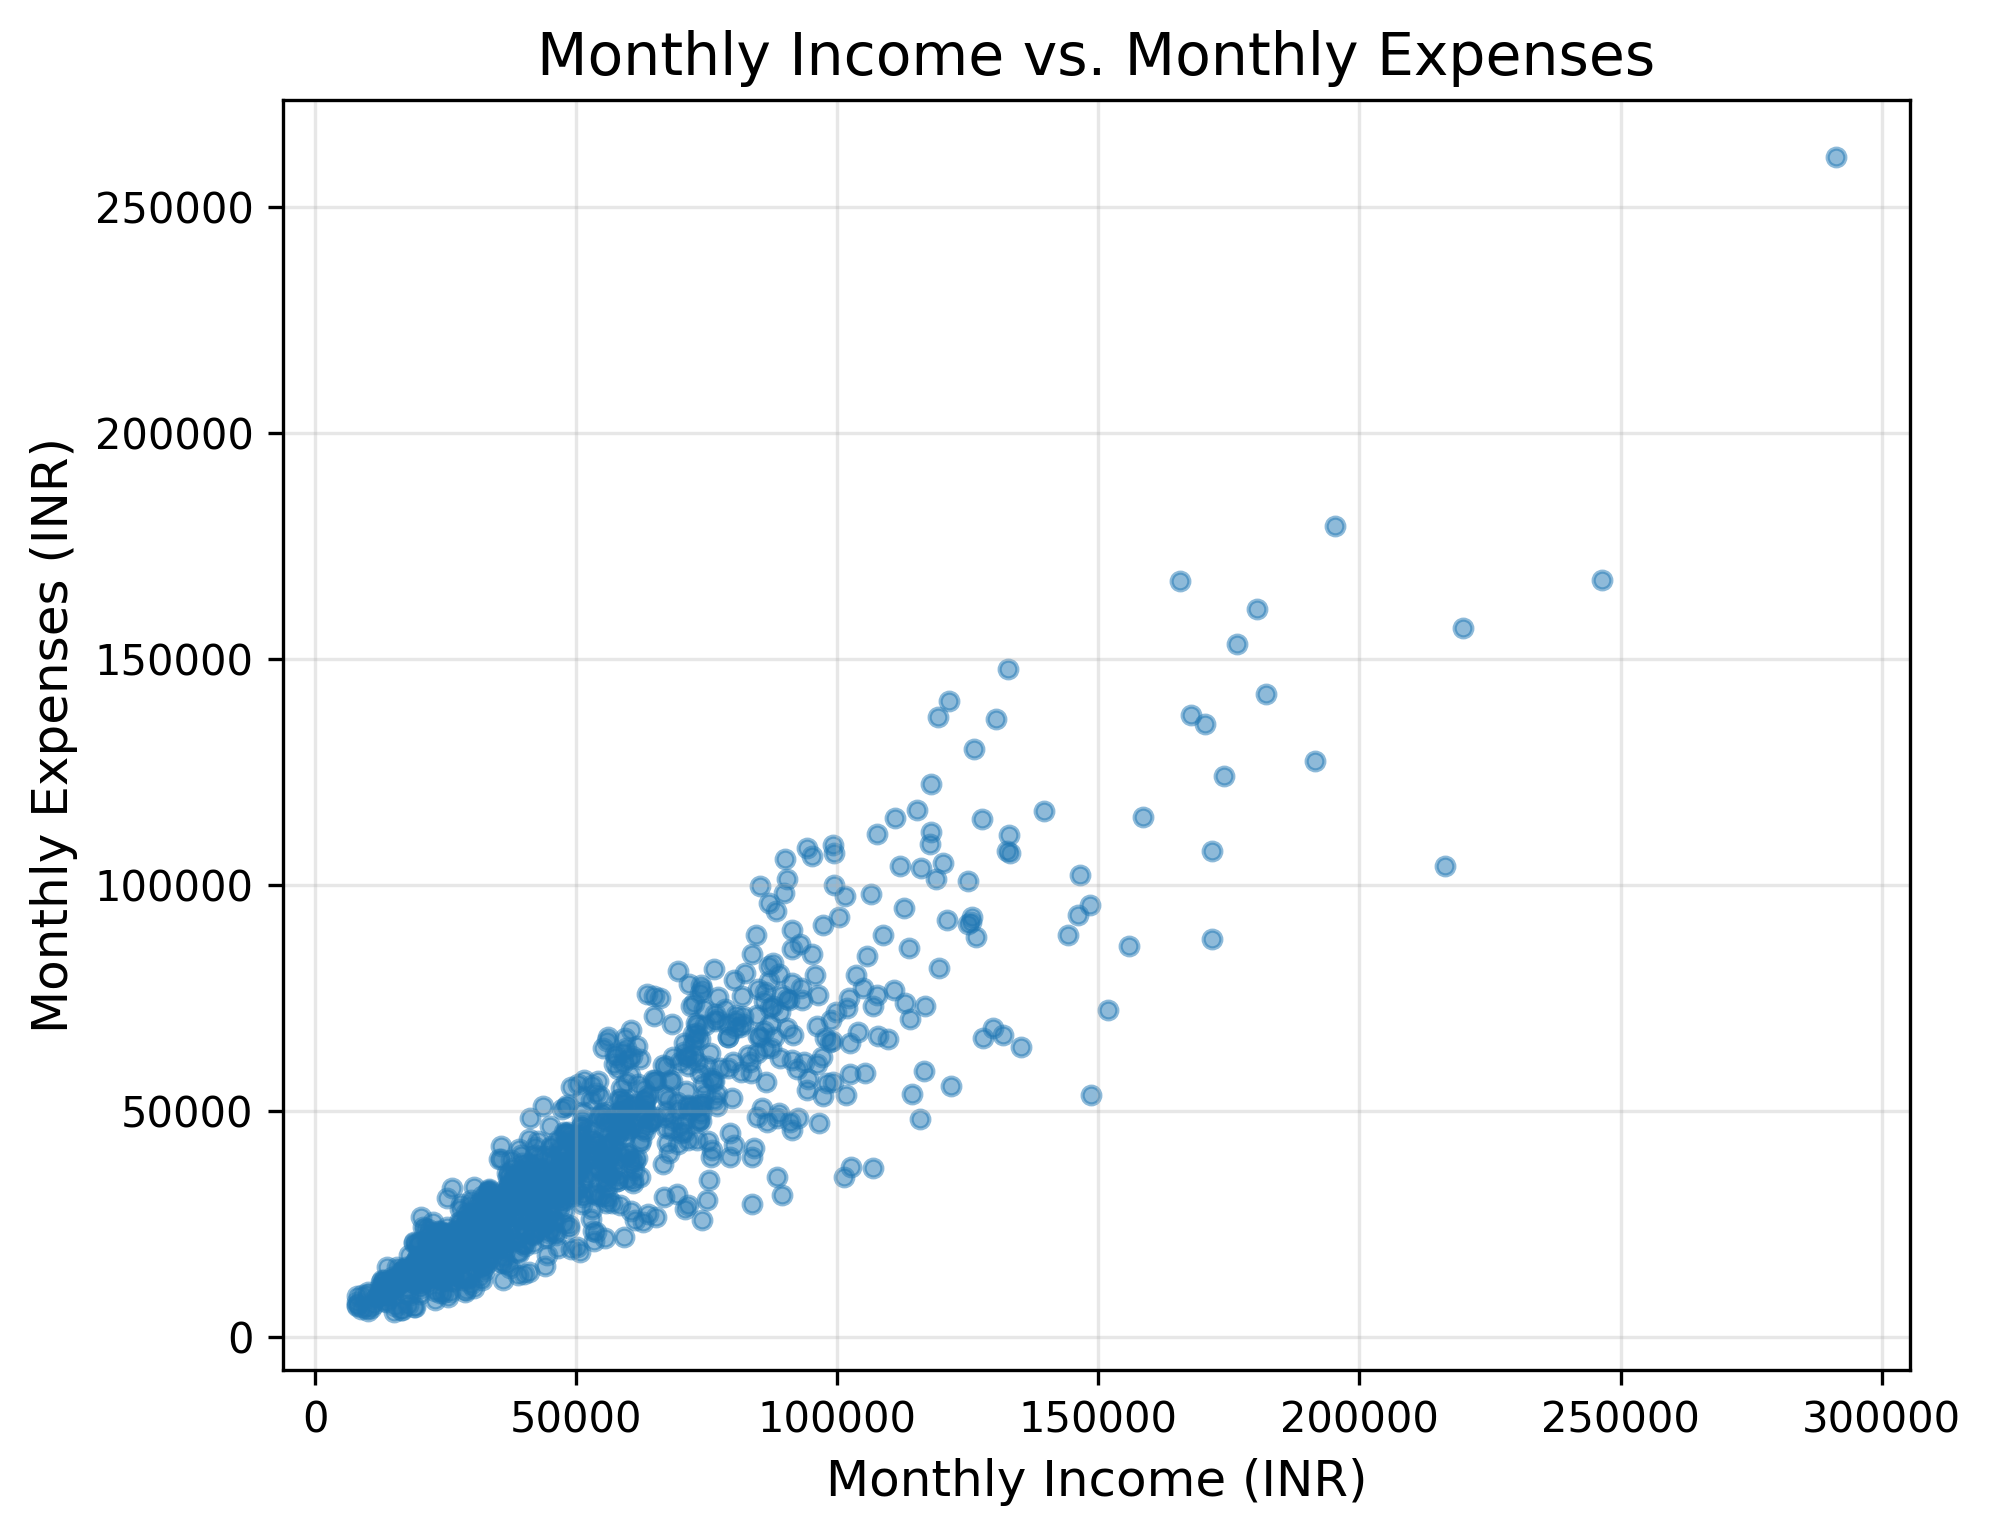
\includegraphics[width=0.78\textwidth]{figures/income_expenses_scatter.png}
    \caption{Monthly income versus monthly expenses for the synthetic user population.}
    \label{fig:income_expenses}
\end{figure}

\clearpage

\begin{figure}[H]
    \centering
    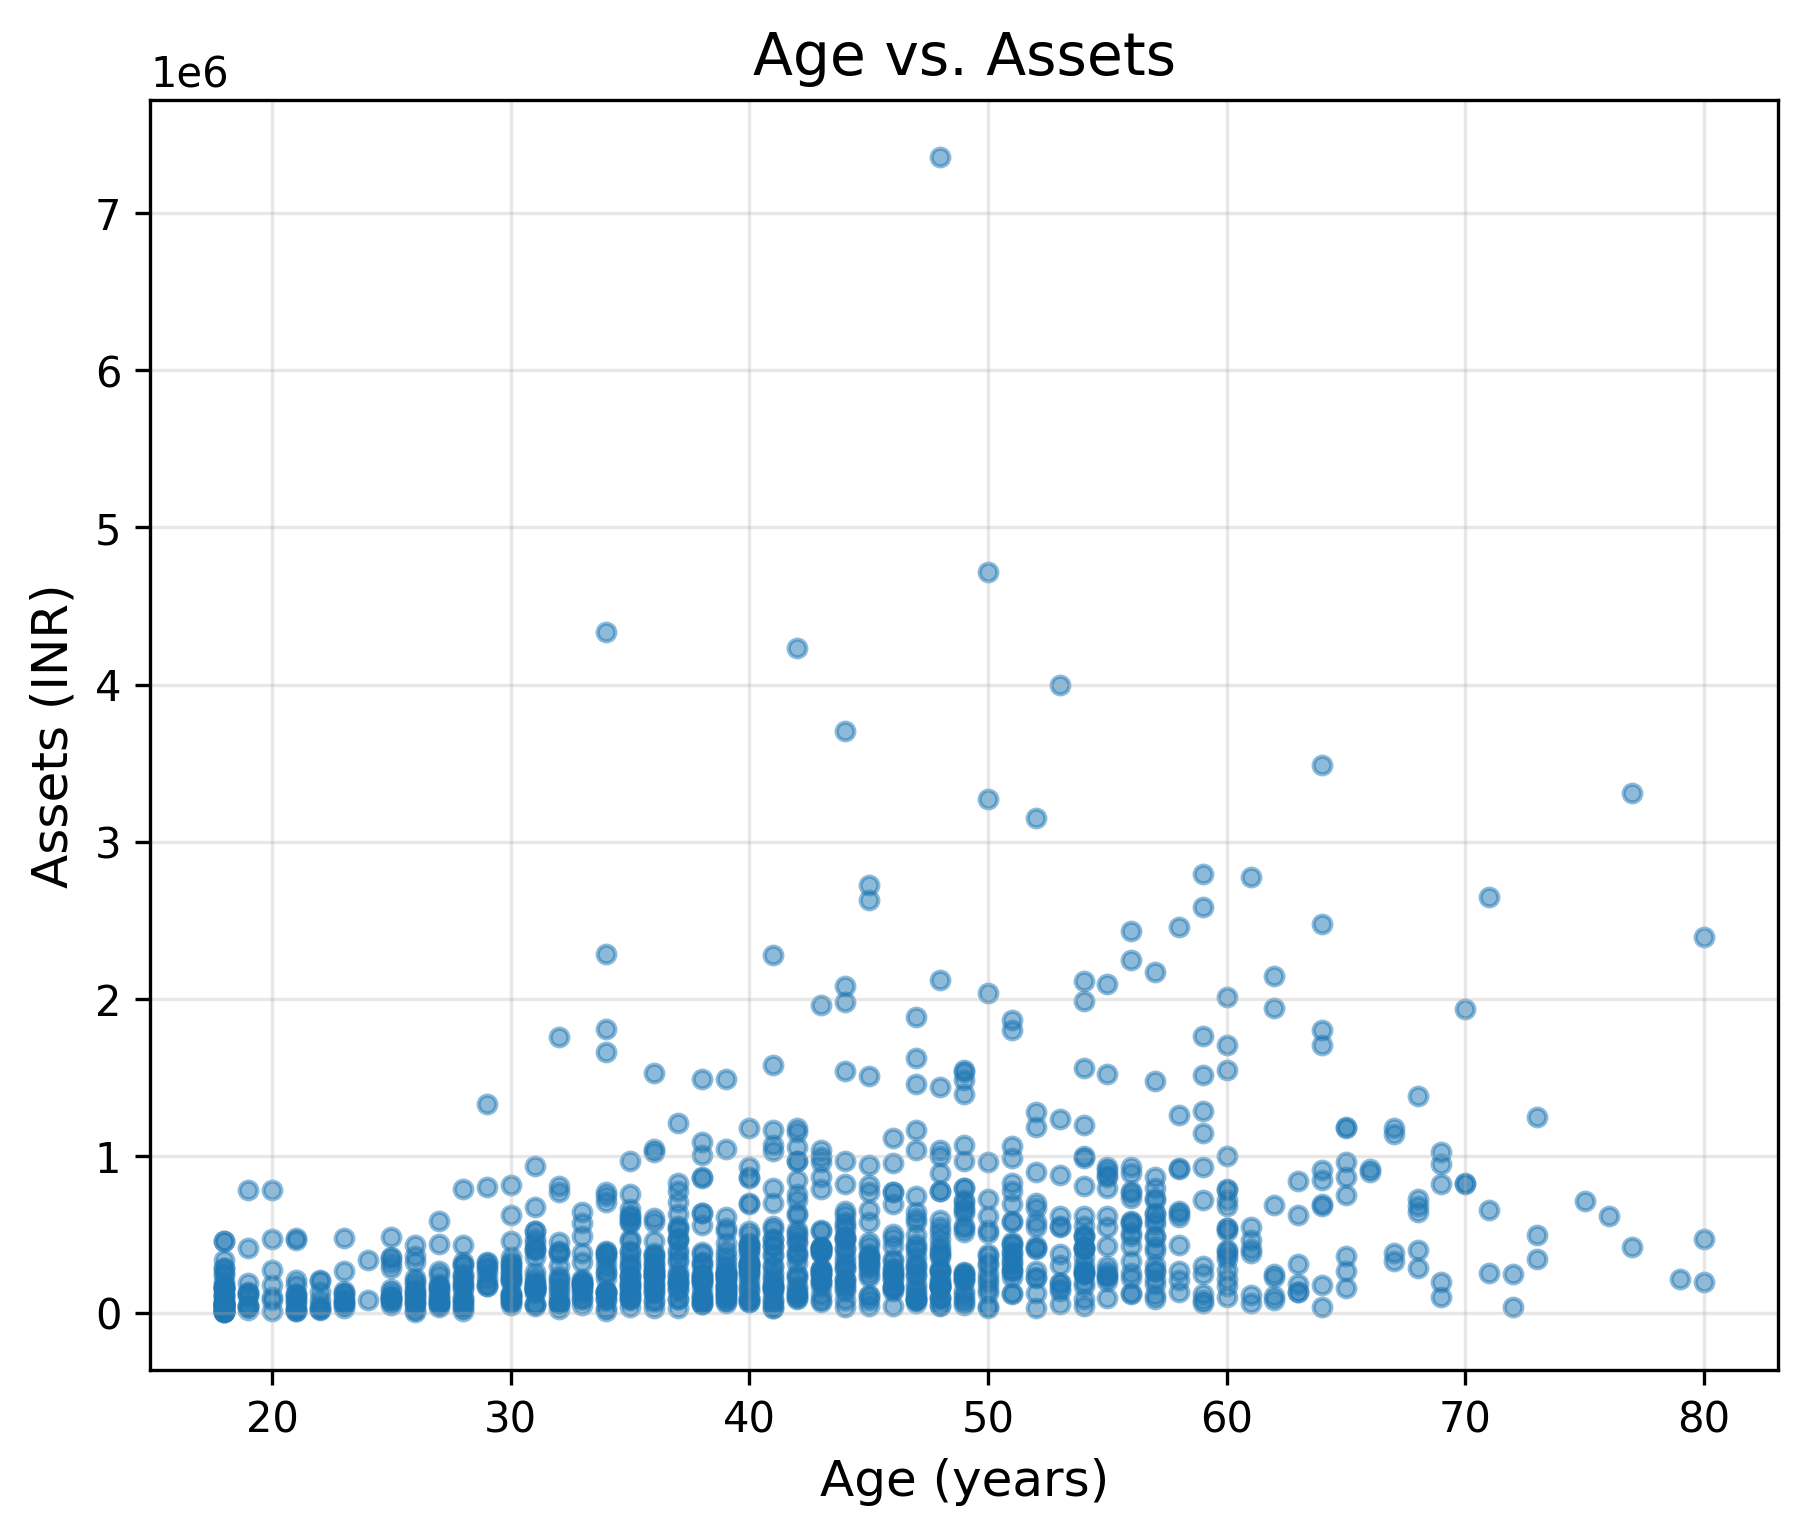
\includegraphics[width=0.78\textwidth]{figures/age_assets_scatter.png}
    \caption{Relationship between user age and total assets.}
    \label{fig:age_assets}
\end{figure}

\clearpage

\begin{figure}[H]
    \centering
    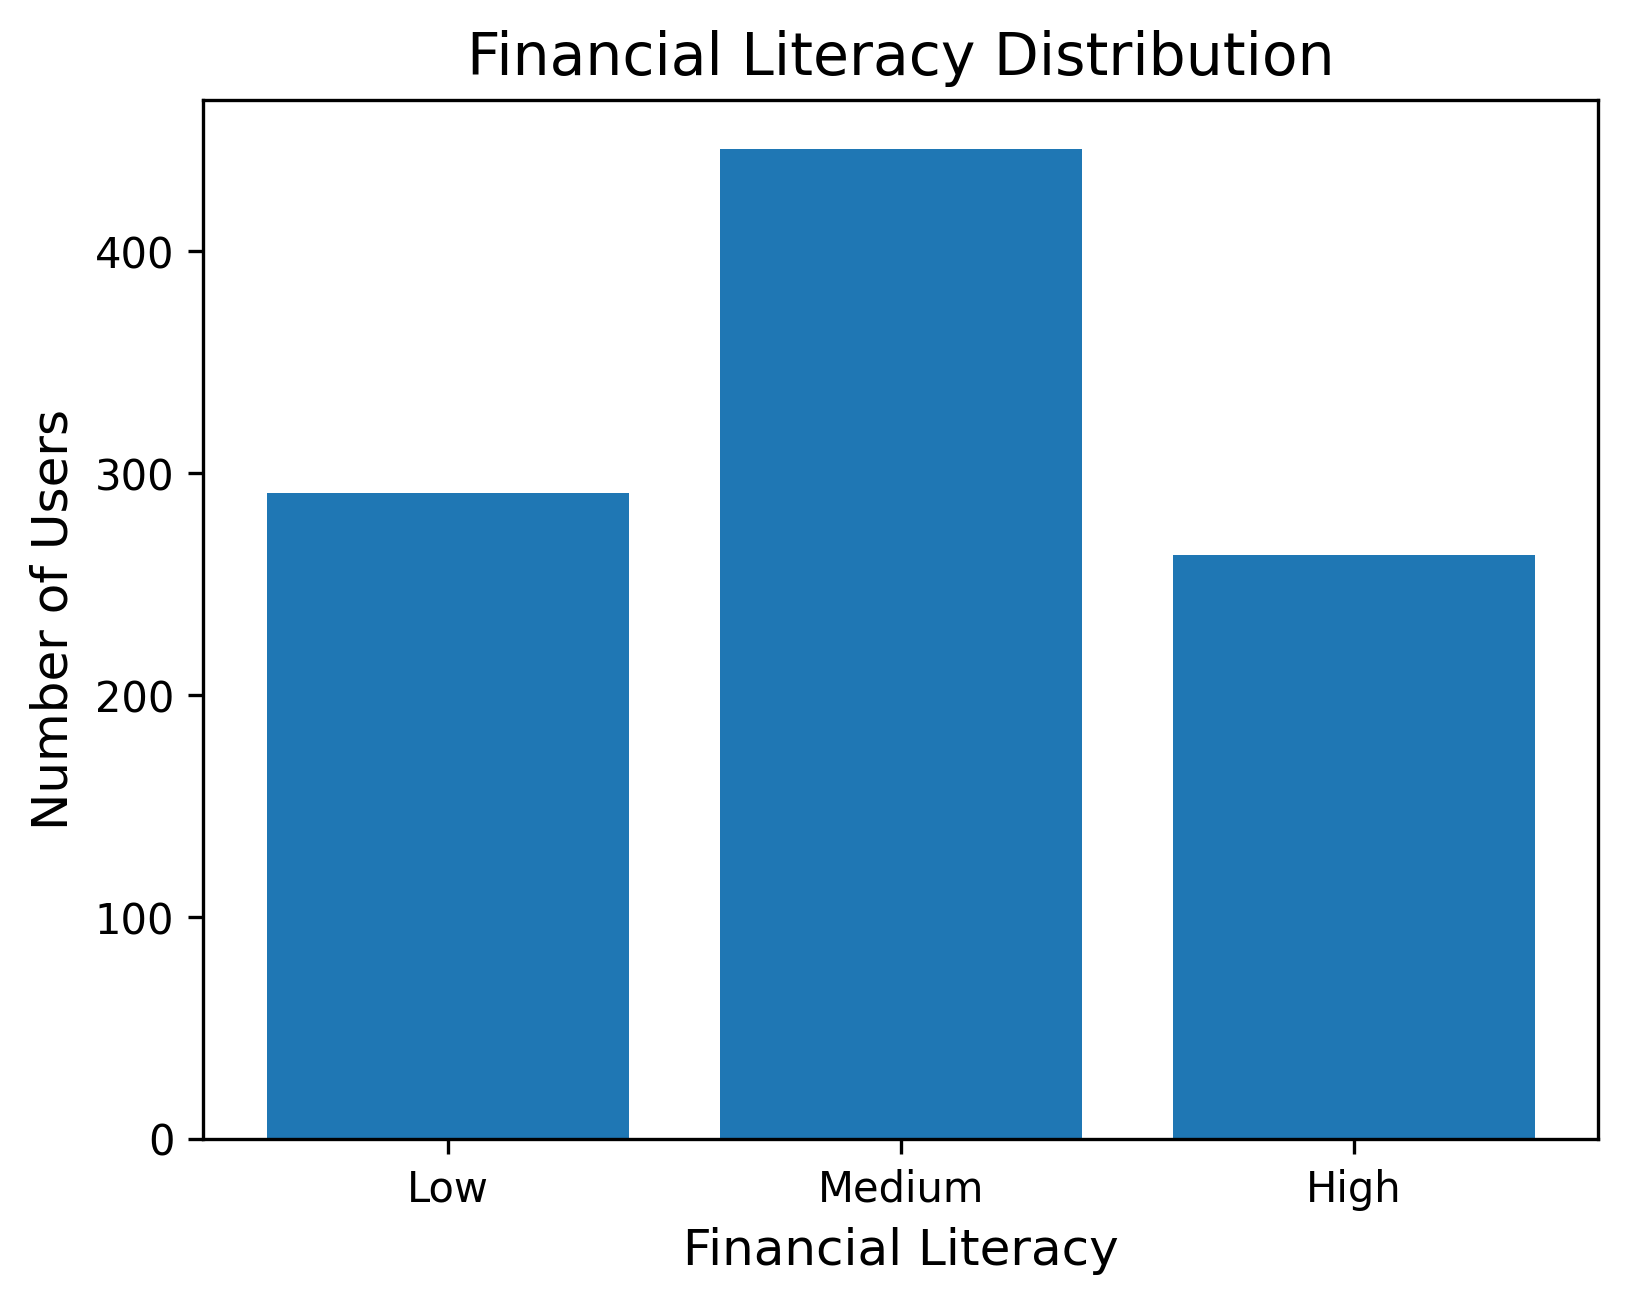
\includegraphics[width=0.78\textwidth]{figures/financial_literacy_distribution.png}
    \caption{Financial literacy distribution among the synthetic users.}
    \label{fig:financial_literacy}
\end{figure}

\clearpage

\begin{figure}[H]
    \centering
    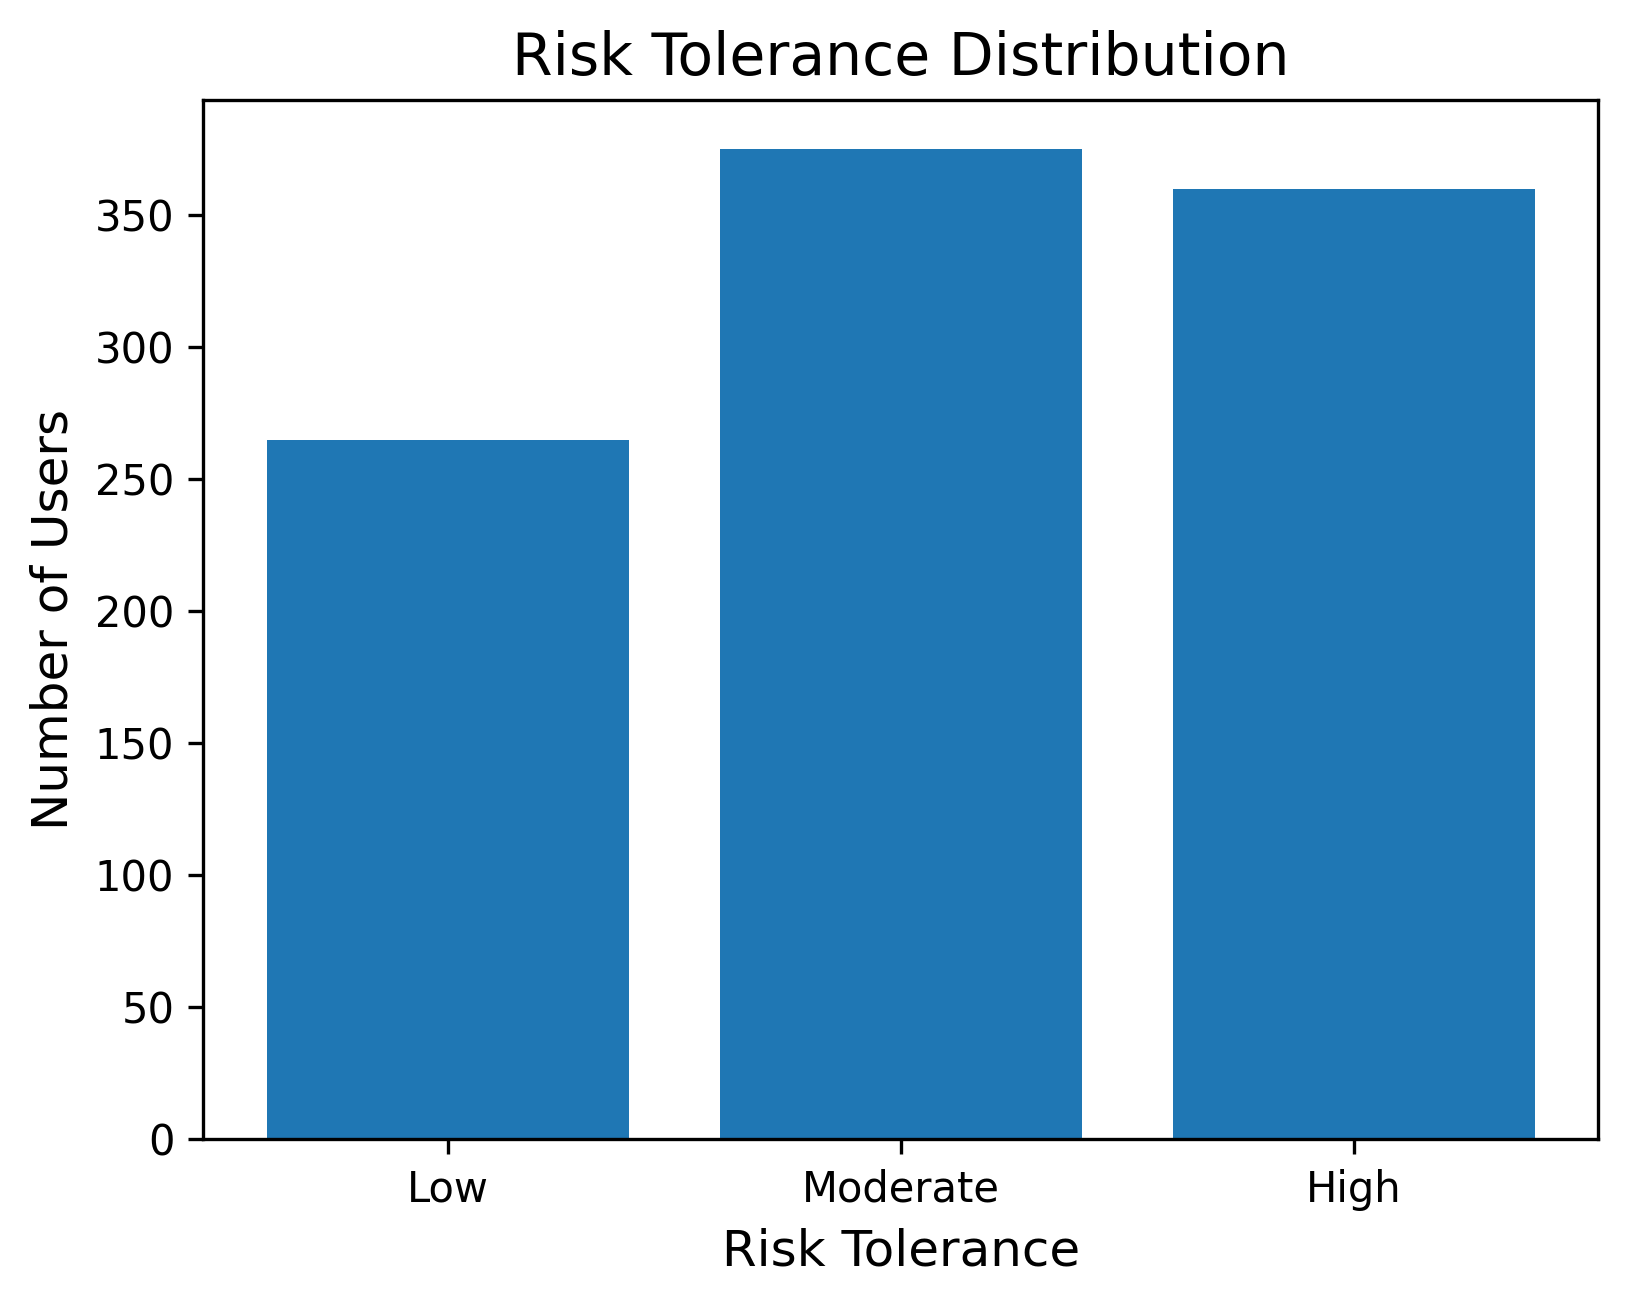
\includegraphics[width=0.78\textwidth]{figures/risk_tolerance_distribution.png}
    \caption{Risk tolerance distribution among the synthetic users.}
    \label{fig:risk_tolerance}
\end{figure}

\clearpage

\begin{figure}[H]
    \centering
    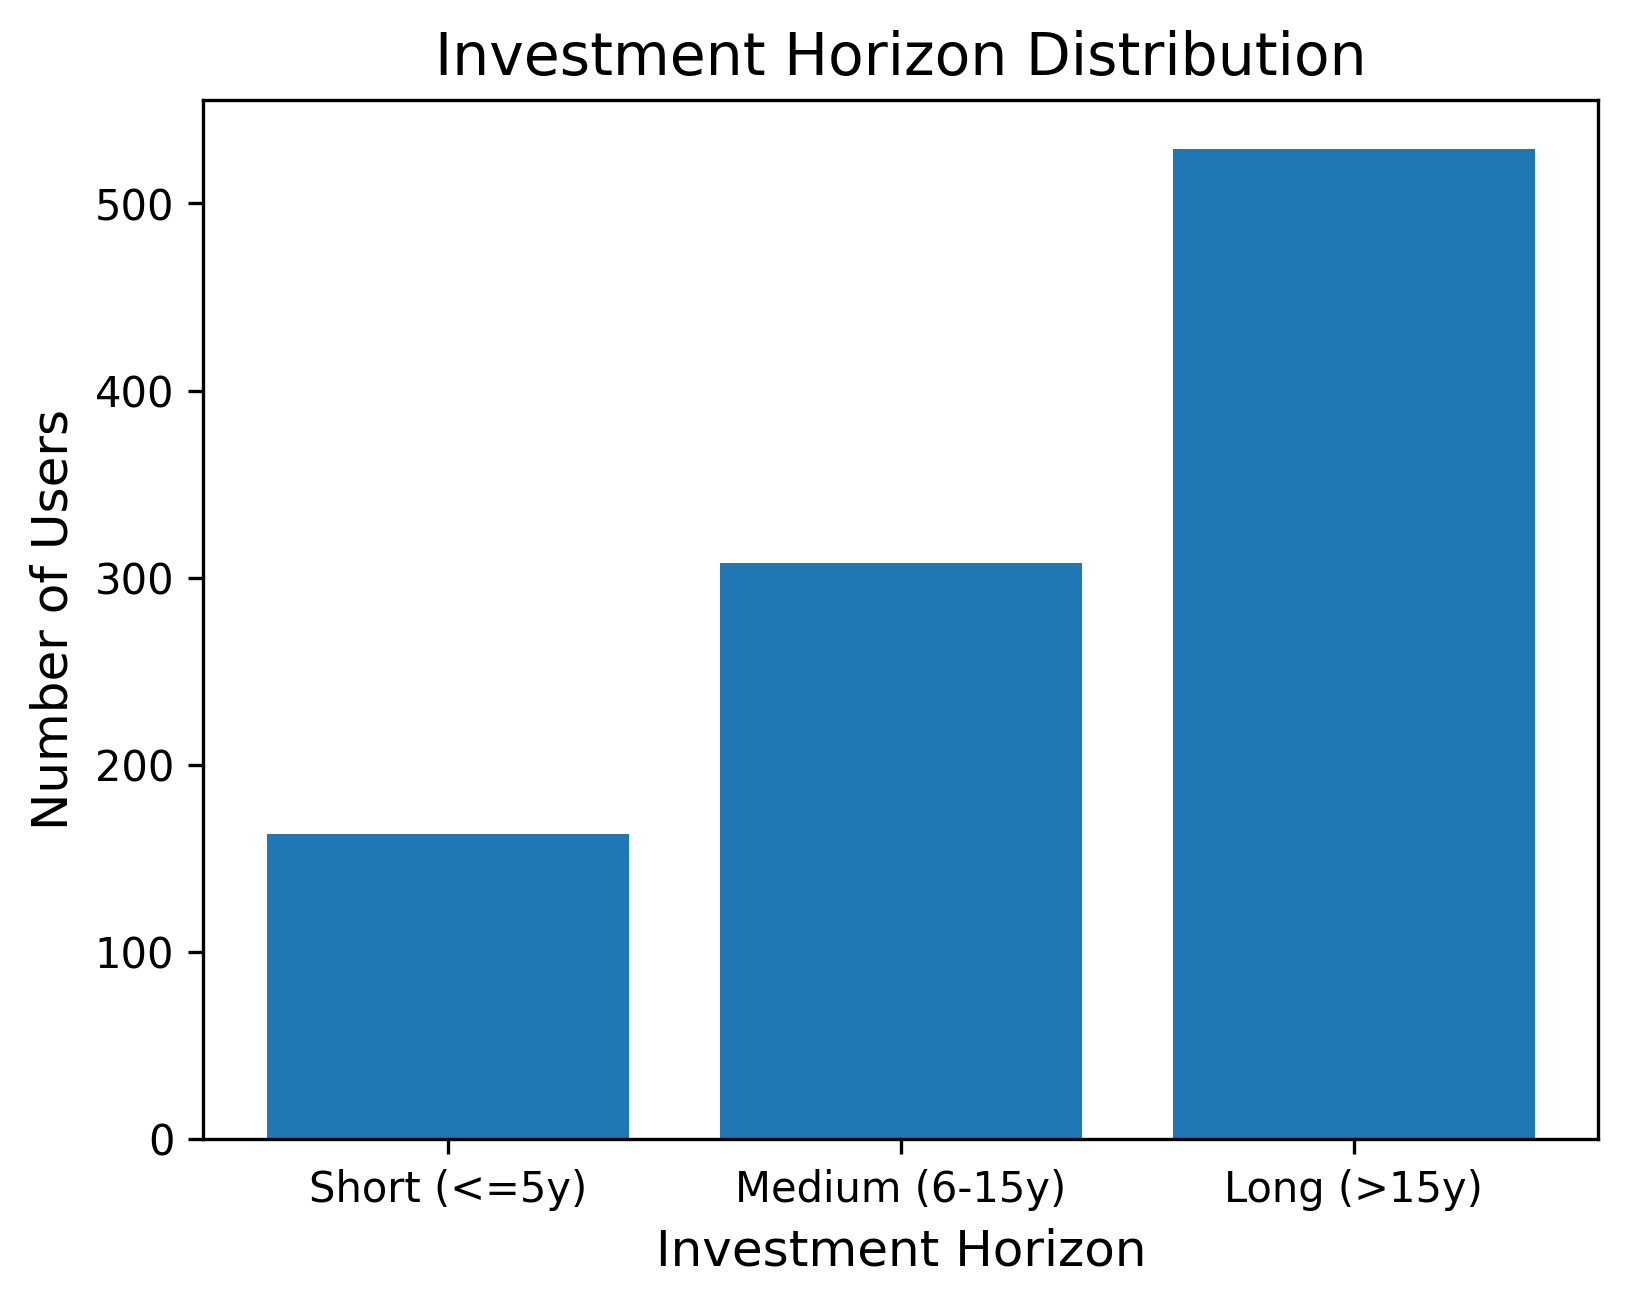
\includegraphics[width=0.78\textwidth]{figures/investment_horizon_distribution.png}
    \caption{Investment horizon distribution among the synthetic users.}
    \label{fig:investment_horizon}
\end{figure}

\clearpage

% =========================================================
\section{Synthetic Scenario Benchmark}

\subsection{Scenario categories}

Each user receives five scenarios, producing 5,000 scenarios in total.

The five categories are:
\begin{enumerate}
    \item Budgeting;
    \item Debt prioritization;
    \item Emergency-fund planning;
    \item Investment allocation; and
    \item Retirement planning.
\end{enumerate}

The scenario generator is implemented in:

\begin{quote}
\texttt{simulations/generate\_scenarios.py}
\end{quote}

The generated scenarios are stored at:

\begin{quote}
\texttt{data/synthetic/scenarios.json}
\end{quote}

\subsection{Scenario design}

The scenarios are template-based and deterministic. They contain both straightforward and under-specified questions.

Straightforward questions may include financial values directly derived from the user's profile. Under-specified questions intentionally omit some numerical information so that later systems can be tested for appropriate clarification or abstention.

No financial value is fabricated for a scenario. The field \texttt{relevant\_user\_attributes} is constructed by copying the corresponding values directly from the user model. The \texttt{required\_information} field is derived from those attributes.

The scenario generator also contains specific protections:
\begin{itemize}
    \item a debt question only references a specific loan if the user has a loan;
    \item a retirement question only references an explicit retirement target if the user has a retirement goal;
    \item scenario identifiers are deterministic and sequential;
    \item the scenario distribution is recorded in metadata; and
    \item the source dataset version and random seed are retained for lineage.
\end{itemize}

\subsection{Scenario validation}

The scenario generator added 17 dedicated tests. Together with the earlier user-generation tests, the benchmark generation stage was validated before the ground-truth engine was introduced. The complete test suite subsequently reached 84 passing tests after the ground-truth implementation and audit, and has since grown to 133 passing tests following the Phase 6A and Phase 6B interface and orchestration work described in Section~\ref{sec:status}.

% =========================================================
\section{Deterministic Ground-Truth Engine}

\subsection{Purpose}

The deterministic ground-truth engine is an independent reference mechanism for evaluating the later language-model systems.

It is important to distinguish this from professional financial advice. The engine represents the expected decision under explicitly defined synthetic benchmark rules. It is therefore an \textbf{evaluation oracle}, not a claim that its rules are universally optimal.

The implementation is located in:

\begin{quote}
\texttt{src/decision/ground\_truth.py}
\end{quote}

Supporting components are:
\begin{itemize}
    \item \texttt{src/decision/candidate\_catalogue.py};
    \item \texttt{src/decision/candidate\_evaluator.py};
    \item \texttt{src/decision/ranking.py}.
\end{itemize}

The resulting benchmark is stored at:

\begin{quote}
\texttt{data/synthetic/ground\_truth.json}
\end{quote}

\subsection{Bounded candidate catalogues}

Each decision category has a bounded catalogue.

\begin{table}[H]
\centering
\caption{Ground-truth candidate decisions}
\label{tab:catalogues}
\begin{tabular}{p{0.25\textwidth}p{0.65\textwidth}}
\toprule
Scenario type & Candidate decisions\\
\midrule
Budgeting & Increase savings; reduce expenses first; maintain current savings; abstain\\
Debt & Invest; repay loan; build emergency fund first; split; abstain\\
Emergency fund & Maintain current; build to 3 months; build to 6 months; build to 9 months; abstain\\
Investment & Conservative; moderate; balanced; growth; aggressive; abstain\\
Retirement & On track; increase retirement saving; extend horizon; reduce target; abstain\\
\bottomrule
\end{tabular}
\end{table}

Bounding the candidate set prevents the reference system from creating an unrestricted recommendation space.

\subsection{Hard constraints}

Candidates are first filtered using hard constraints. A candidate that violates a mandatory condition cannot be selected merely because it receives a high soft score.

This produces an explicit distinction between:
\begin{quote}
\textbf{candidate is infeasible}
\end{quote}
and
\begin{quote}
\textbf{candidate is feasible but less suitable}.
\end{quote}

This distinction will later support faithful explanation because the system can record which constraint eliminated an alternative.

\subsection{Ranking hierarchy}

After hard-constraint filtering, candidates are ranked using the following deterministic hierarchy:

\begin{enumerate}
    \item eliminate hard-constraint violations;
    \item maximize goal alignment;
    \item minimize suitability risk;
    \item maximize financial objective score;
    \item maximize liquidity preservation;
    \item use fixed catalogue order as the deterministic final tie-break.
\end{enumerate}

This hierarchy was selected to ensure that mandatory suitability requirements take precedence over attractive numerical outcomes.

\subsection{Abstention}

Abstention is explicitly represented rather than treated as a failure.

The engine can abstain when:
\begin{itemize}
    \item required information is missing;
    \item no valid candidate remains;
    \item an unsupported scenario is encountered;
    \item a required tool is unavailable in future tool-based extensions; or
    \item another explicitly defined abstention condition is triggered.
\end{itemize}

Some abstention reasons are currently structurally unreachable in the deterministic benchmark because the scenario catalogue and scoring engine form a closed system. These reasons remain documented so that the architecture can support future extensions.

\subsection{Current ground-truth output}

The final ground-truth dataset contains exactly 5,000 records.

\begin{table}[H]
\centering
\caption{Ground-truth decision distribution}
\label{tab:gt}
\begin{tabular}{llr}
\toprule
Scenario & Decision & Count\\
\midrule
Budgeting & Increase savings & 748\\
Budgeting & Reduce expenses first & 246\\
Budgeting & Maintain current savings & 6\\
\midrule
Debt & Invest & 566\\
Debt & Repay loan & 175\\
Debt & Build emergency fund first & 233\\
Debt & Split & 1\\
Debt & Abstain & 25\\
\midrule
Emergency & Maintain current & 347\\
Emergency & Build to 3 months & 291\\
Emergency & Build to 6 months & 263\\
Emergency & Build to 9 months & 99\\
\midrule
Investment & Conservative & 255\\
Investment & Moderate & 39\\
Investment & Balanced & 328\\
Investment & Growth & 31\\
Investment & Aggressive & 347\\
\midrule
Retirement & On track & 371\\
Retirement & Increase retirement saving & 221\\
Retirement & Extend horizon & 220\\
Retirement & Reduce target & 188\\
\bottomrule
\end{tabular}
\end{table}

The distribution is intentionally not forced to be uniform. It reflects the current synthetic population and the deterministic scoring rules.

\subsection{Investment distribution audit}

During validation, the investment decision distribution revealed an important methodological issue. Moderate and growth candidates were initially almost unreachable.

A cross-tabulation of risk tolerance and investment horizon showed that the synthetic population had a very strong structural relationship between these two fields. In particular, some combinations required by the candidate scoring rules did not occur in the population.

The issue was therefore diagnosed as a population-generation problem rather than simply changing thresholds until the distribution looked uniform.

A small secondary adjustment using financial literacy was introduced because financial literacy is independently generated from risk tolerance and investment horizon in the synthetic population. The adjustment was limited to a small range and documented as a suitability factor.

The resulting investment distribution became:

\begin{itemize}
    \item Conservative: 255;
    \item Moderate: 39;
    \item Balanced: 328;
    \item Growth: 31;
    \item Aggressive: 347.
\end{itemize}

All five candidates are now reachable without artificially forcing equal class frequencies.

\subsection{Ground-truth assumptions}

The ground-truth engine contains simplified benchmark assumptions. These include:
\begin{itemize}
    \item a minimum actionable amount of INR 1,000 for certain decisions;
    \item retirement nominal return assumptions of 4\%, 7\%, and 10\% for low, moderate, and high risk categories;
    \item a 10-times-annual-income fallback retirement target when an explicit retirement target is unavailable; and
    \item simplified suitability and liquidity scoring formulas.
\end{itemize}

These are explicitly documented as \textbf{synthetic benchmark assumptions, not financial advice}. They are used to produce a deterministic evaluation reference and should not be presented as validated investment or retirement recommendations.

% =========================================================
\section{Simulation Validation and Reproducibility}

Reproducibility is a core requirement of the benchmark.

The primary dataset uses:
\begin{itemize}
    \item Random seed: 42;
    \item Users: 1,000;
    \item Scenarios: 5,000;
    \item Ground-truth records: 5,000.
\end{itemize}

The user and scenario generators use deterministic seeded random generation. The scenario generator uses a local random-number generator so that its output is not affected by random-number consumption elsewhere in the program.

The ground-truth engine is deterministic with respect to the user and scenario inputs.

A complete regeneration of the ground-truth dataset was performed and produced byte-identical records and metadata, excluding generation timestamps. The summary output was also identical.

The benchmark source files were kept read-only during ground-truth generation. This was explicitly tested by confirming that the user and scenario files were not modified.

\subsection{Test-suite and reproducibility evidence}

The claims above are not asserted without evidence. The automated test suite was re-run and the ground-truth dataset was independently regenerated and diffed against the committed copy immediately before this report was finalized; the actual terminal output is reproduced below.

\begin{quote}
\texttt{\$ python -m pytest -q}
\end{quote}
{\small
\begin{verbatim}
........................................................................ [ 54%]
.............................................................            [100%]
133 passed in 9.27s
\end{verbatim}
}

\begin{quote}
\texttt{\$ python -m src.decision.ground\_truth --output ...\_verify.json}\\
\texttt{\$ python -c "compare ground\_truth.json against ..\_verify.json"}
\end{quote}
{\small
\begin{verbatim}
records identical: True
metadata (excl generated_at) identical: True
users.json generated_at unchanged: 2026-09-11T17:07:41.252516+00:00
scenarios.json generated_at unchanged: 2026-09-11T17:28:01.134520+00:00
\end{verbatim}
}

This confirms, from an independently re-run regeneration rather than from the original generation run alone, that (i) the full 133-test suite passes, (ii) the ground-truth engine produces byte-identical output from the same seed-42 source files, and (iii) neither \texttt{users.json} nor \texttt{scenarios.json} was modified as a side effect of generating ground truth. Section~\ref{sec:evidence-records} reproduces the underlying records this evidence refers to.

% =========================================================
\section{Software Architecture and Repository Structure}

The implementation is organized so that benchmark generation, deterministic decision logic, experiment orchestration, and later LLM components remain separate.

\begin{verbatim}
financial-copilot/
|
+-- configs/
|   +-- baseline.yaml
|   +-- rag.yaml
|   +-- personalized.yaml
|   +-- full_copilot.yaml
|
+-- data/
|   +-- synthetic/
|       +-- users.json
|       +-- scenarios.json
|       +-- ground_truth.json
|       +-- experiment_manifest.json
|
+-- simulations/
|   +-- generate_users.py
|   +-- generate_scenarios.py
|
+-- src/
|   +-- models/
|   +-- decision/
|   +-- agents/
|   +-- retrieval/
|   +-- personalization/
|   +-- constraints/
|   +-- tools/
|   +-- explanation/
|   +-- audit/
|   +-- evaluation/
|
+-- experiments/
|   +-- run_experiment.py
|   +-- manifest.py
|
+-- visualizations/
|   +-- generate_user_plots.py
|
+-- tests/
|
+-- results/
|   +-- raw/
|   +-- metrics/
|   +-- tables/
|   +-- figures/
|
+-- docs/
|
+-- README.md
\end{verbatim}

The separation of \texttt{src/decision/} from future LLM components is particularly important. It prevents the model being evaluated from defining its own reference answer. Similarly, \texttt{experiments/} only dispatches to the frozen agent interfaces in \texttt{src/agents/} and never re-implements ranking or scoring logic.

\subsection{GitHub / Source Code}

The complete implementation will be maintained in the project's GitHub repository.

\begin{quote}
\textbf{GitHub Repository:} \url{INSERT-YOUR-GITHUB-REPOSITORY-LINK-HERE}
\end{quote}

\textbf{Replace the placeholder above with the final public/private repository URL.}

Recommended repository resources to document in the final version include:
\begin{itemize}
    \item source code;
    \item synthetic dataset generation scripts;
    \item generated benchmark files;
    \item test suite;
    \item experiment configuration files;
    \item result files;
    \item architecture diagrams;
    \item README and setup instructions; and
    \item final experiment commands.
\end{itemize}

% =========================================================
\section{Experimental Configurations}

The next implementation stage compares four configurations using the same benchmark. Section~\ref{sec:status} describes what is currently implemented for each.

\subsection{Configuration A: Baseline LLM}

The baseline receives the financial question and produces a recommendation and natural-language explanation.

It does not receive the complete personalization, retrieval, deterministic-tool, and constraint pipeline.

The purpose is to establish the performance of a relatively unconstrained generative approach.

\subsection{Configuration B: Retrieval-Augmented Generation}

The RAG configuration introduces external evidence retrieval.

The purpose is to evaluate whether grounding the generation process in retrievable evidence improves factual correctness and explanation support.

\subsection{Configuration C: Personalized LLM}

The personalized configuration receives the scenario together with the user's financial profile.

This configuration tests whether explicit user context improves the suitability of the recommendation.

\subsection{Configuration D: Full Financial Copilot}

The proposed full configuration combines:
\begin{itemize}
    \item personalization;
    \item retrieval;
    \item bounded candidate catalogues;
    \item deterministic financial tools;
    \item hard constraint filtering;
    \item candidate ranking;
    \item deterministic confidence;
    \item abstention;
    \item artifact-grounded explanation; and
    \item audit logging.
\end{itemize}

\begin{figure}[H]
\centering
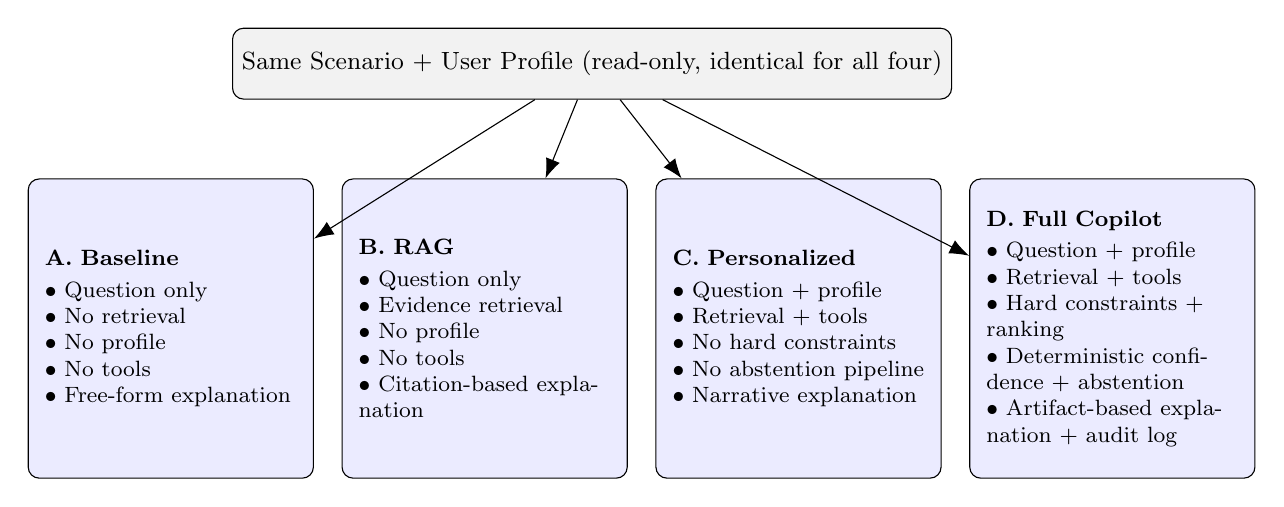
\begin{tikzpicture}[
    inputbox/.style={rectangle, draw, rounded corners, minimum width=8cm, minimum height=0.9cm, align=center, font=\small, fill=gray!10},
    cfgcol/.style={rectangle, draw, rounded corners, text width=3.2cm, minimum height=3.8cm, align=left, font=\footnotesize, fill=blue!8, inner sep=6pt},
    node distance=0.5cm
]
\node[inputbox] (input) {Same Scenario + User Profile (read-only, identical for all four)};

\node[cfgcol, below=1.0cm of input, xshift=-5.35cm] (A) {
    \textbf{A. Baseline}\\[2pt]
    $\bullet$ Question only\\
    $\bullet$ No retrieval\\
    $\bullet$ No profile\\
    $\bullet$ No tools\\
    $\bullet$ Free-form explanation
};
\node[cfgcol, right=0.35cm of A] (B) {
    \textbf{B. RAG}\\[2pt]
    $\bullet$ Question only\\
    $\bullet$ Evidence retrieval\\
    $\bullet$ No profile\\
    $\bullet$ No tools\\
    $\bullet$ Citation-based explanation
};
\node[cfgcol, right=0.35cm of B] (C) {
    \textbf{C. Personalized}\\[2pt]
    $\bullet$ Question + profile\\
    $\bullet$ Retrieval + tools\\
    $\bullet$ No hard constraints\\
    $\bullet$ No abstention pipeline\\
    $\bullet$ Narrative explanation
};
\node[cfgcol, right=0.35cm of C] (D) {
    \textbf{D. Full Copilot}\\[2pt]
    $\bullet$ Question + profile\\
    $\bullet$ Retrieval + tools\\
    $\bullet$ Hard constraints + ranking\\
    $\bullet$ Deterministic confidence + abstention\\
    $\bullet$ Artifact-based explanation + audit log
};

\draw[-{Latex[length=2.5mm]}] (input) -- (A);
\draw[-{Latex[length=2.5mm]}] (input) -- (B);
\draw[-{Latex[length=2.5mm]}] (input) -- (C);
\draw[-{Latex[length=2.5mm]}] (input) -- (D);
\end{tikzpicture}
\caption{Controlled comparison of the four experimental configurations. All four receive an identical, unmodified scenario -- the baseline never receives hidden user information, and the personalized/full configurations receive profile information only through the explicitly permitted interface.}
\label{fig:configs}
\end{figure}

% =========================================================
\section{Evaluation Methodology}

\subsection{D1 -- Correctness}

The primary correctness measure will compare the system's decision with the deterministic ground-truth decision.

Additional measures may include:
\begin{itemize}
    \item numerical calculation accuracy;
    \item hallucination rate;
    \item evidence correctness;
    \item citation correctness; and
    \item abstention correctness.
\end{itemize}

\subsection{D2 -- Explanation Faithfulness}

Faithfulness is evaluated separately from correctness.

The planned perturbation tests include:

\textbf{Evidence removal:} remove evidence cited or supplied to the system and determine whether the recommendation changes when that evidence is genuinely decision-relevant.

\textbf{Evidence corruption:} alter an evidence value and determine whether the resulting recommendation responds appropriately while checking whether the explanation accurately reflects the evidence actually used.

\textbf{Tool-output perturbation:} modify a deterministic tool result and test whether the recommendation responds consistently.

\textbf{Constraint perturbation:} change a user's binding constraint and determine whether the recommendation and explanation respond to that change.

\textbf{Explanation/artifact consistency:} verify that statements made in the user-facing explanation are supported by the stored evidence, tool outputs, constraints, and decision artifacts.

An important methodological distinction is:

\begin{quote}
\textbf{Correctness asks whether the recommendation is right under the benchmark. Faithfulness asks whether the explanation accurately represents the artifacts and factors actually used by the system.}
\end{quote}

A deliberately corrupted input may therefore produce an incorrect recommendation while still producing a faithful explanation of what the system actually observed.

\subsection{D3 -- Personalization Quality}

Personalization will be evaluated using:
\begin{itemize}
    \item preference and constraint elicitation accuracy;
    \item suitability-violation rate; and
    \item profile sensitivity.
\end{itemize}

Profile sensitivity will use controlled counterfactual user profiles. For example, investment horizon, risk tolerance, liquidity requirement, or debt burden can be changed while other variables remain fixed. The system should respond when the changed attribute is decision-relevant.

\subsection{D4 -- Abstention}

The system should abstain rather than fabricate a recommendation when:
\begin{itemize}
    \item required information is missing;
    \item evidence required for a grounded answer is unavailable;
    \item a required tool fails;
    \item no valid candidate remains;
    \item the scenario is unsupported; or
    \item confidence is insufficient under the defined deterministic confidence policy.
\end{itemize}

Abstention will therefore be evaluated using both:
\begin{itemize}
    \item unsafe recommendation rate; and
    \item abstention precision/recall.
\end{itemize}

\subsection{D5 -- Governance and Auditability}

Governance evaluation will examine:
\begin{itemize}
    \item audit completeness;
    \item evidence provenance;
    \item tool-call trace completeness;
    \item constraint-binding records;
    \item rejected-candidate records;
    \item reproducibility of a decision from the stored log; and
    \item human oversight/interruption points.
\end{itemize}

% =========================================================
\section{Current Implementation Status}
\label{sec:status}

The current project status is summarized below.

\begin{table}[H]
\centering
\caption{Implementation status at the time of this report}
\label{tab:status}
\begin{tabular}{p{0.65\textwidth}p{0.20\textwidth}}
\toprule
Component & Status\\
\midrule
Literature review & Complete\\
Research gaps & Complete\\
Five-layer architecture & Designed\\
Synthetic user generator & Complete\\
Synthetic user dataset & Complete\\
Scenario generator & Complete\\
Scenario benchmark & Complete\\
Deterministic candidate catalogue & Complete\\
Ground-truth engine & Complete\\
Ground-truth audit & Complete\\
Benchmark reproducibility validation & Complete\\
Phase 6A experimental interfaces (common input/output contract) & Complete\\
Phase 6B execution/orchestration layer & Complete\\
Baseline LLM (real model call) & Pending (stub only)\\
RAG configuration (real retrieval) & Pending (stub only)\\
Personalized configuration (real personalization) & Pending (stub only)\\
Full financial copilot (real reasoning) & Pending (stub only)\\
Faithfulness experiments & Pending\\
Final comparative evaluation & Pending\\
\bottomrule
\end{tabular}
\end{table}

The benchmark, ground-truth, experiment-contract, and orchestration implementation currently pass:

\begin{center}
\Large\textbf{133 / 133 automated tests}
\end{center}

This is a software-validation result, not an LLM performance result. All four configurations currently execute only clearly-labeled placeholder logic (Phase 6A/6B stubs) that satisfies the frozen input/output contract; none yet calls a language model, retrieval index, or financial tool.

% =========================================================
\section{Expected Experimental Results}

At the current stage, no comparative LLM results are claimed because the four experimental configurations have not yet completed their evaluation runs.

The expected final results section will compare the four configurations across a common set of metrics.

\begin{table}[H]
\centering
\caption{Planned final comparison table}
\label{tab:finalplanned}
\begin{tabular}{lcccc}
\toprule
Metric & Baseline & RAG & Personalized & Full Copilot\\
\midrule
Decision accuracy & TBD & TBD & TBD & TBD\\
Numerical accuracy & TBD & TBD & TBD & TBD\\
Hallucination rate & TBD & TBD & TBD & TBD\\
Faithfulness score & TBD & TBD & TBD & TBD\\
Suitability violations & TBD & TBD & TBD & TBD\\
Profile sensitivity & TBD & TBD & TBD & TBD\\
Unsafe recommendation rate & TBD & TBD & TBD & TBD\\
Abstention precision & TBD & TBD & TBD & TBD\\
Audit completeness & TBD & TBD & TBD & TBD\\
Reproducibility & TBD & TBD & TBD & TBD\\
\bottomrule
\end{tabular}
\end{table}

This table is intentionally left as \texttt{TBD}. It should only be populated after the Phase 7 experiments (the actual language-model, retrieval, and tool implementations) have been executed.

% =========================================================
\section{Planned Explanation Artifact Flow}

The proposed explanation mechanism separates the communication artifact shown to the user from the audit artifact stored by the system.

\begin{figure}[H]
\centering
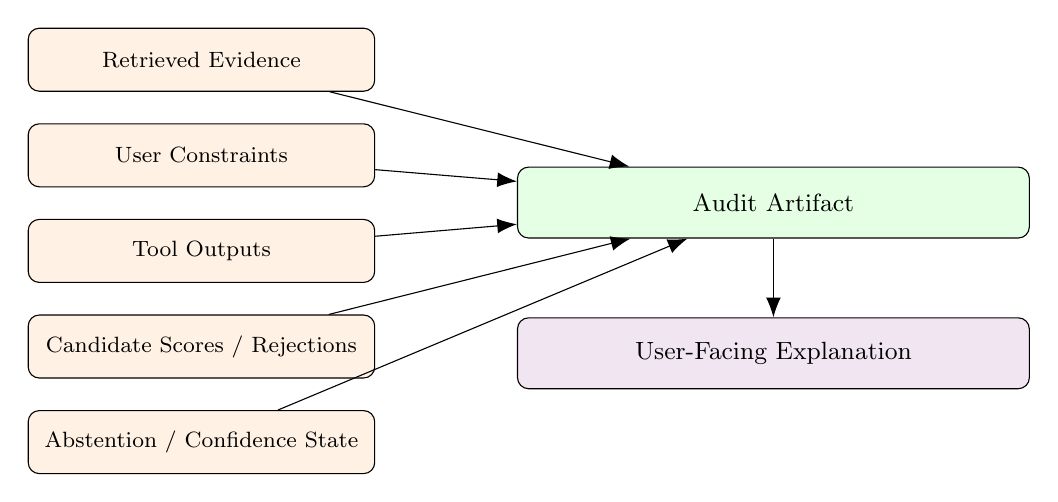
\begin{tikzpicture}[
    src/.style={rectangle, draw, rounded corners, minimum width=4.4cm, minimum height=0.8cm, align=center, font=\footnotesize, fill=orange!10},
    mid/.style={rectangle, draw, rounded corners, minimum width=6.5cm, minimum height=0.9cm, align=center, font=\small, fill=green!10},
    node distance=0.4cm
]
\node[src] (ev) {Retrieved Evidence};
\node[src, below=of ev] (con) {User Constraints};
\node[src, below=of con] (tool) {Tool Outputs};
\node[src, below=of tool] (cand) {Candidate Scores / Rejections};
\node[src, below=of cand] (conf) {Abstention / Confidence State};

\node[mid, right=1.8cm of con, yshift=-0.6cm] (audit) {Audit Artifact};
\node[mid, below=1.0cm of audit, fill=violet!10] (comm) {User-Facing Explanation};

\draw[-{Latex[length=2.5mm]}] (ev) -- (audit);
\draw[-{Latex[length=2.5mm]}] (con) -- (audit);
\draw[-{Latex[length=2.5mm]}] (tool) -- (audit);
\draw[-{Latex[length=2.5mm]}] (cand) -- (audit);
\draw[-{Latex[length=2.5mm]}] (conf) -- (audit);
\draw[-{Latex[length=2.5mm]}] (audit) -- (comm);
\end{tikzpicture}
\caption{Proposed artifact-grounded explanation flow: the user-facing explanation is rendered from the audit artifact and is never generated independently of it.}
\label{fig:explanation}
\end{figure}

The intended design is that the user-facing explanation is a communication layer over verifiable artifacts rather than an independent narrative generated without reference to the actual decision trace.

% =========================================================
\section{Limitations}

The current work has several limitations.

\subsection{Synthetic population}

The benchmark is synthetic and therefore cannot establish that its distributions represent real households. Its purpose is controlled experimentation and reproducibility.

\subsection{Simplified ground truth}

The ground-truth engine uses explicit heuristic formulas. These rules are useful for controlled evaluation but are not validated financial planning rules.

\subsection{Limited decision categories}

The current benchmark contains five decision categories. Other household decisions, such as insurance selection, tax planning, mortgage refinancing, and detailed estate planning, are outside the current scope.

\subsection{No current real-market dataset}

The current benchmark does not use a real financial market dataset or real customer-account dataset. If the final research scope requires current market information, an additional external evidence corpus may be introduced during the grounding/RAG phase.

\subsection{LLM experiments are incomplete}

At the time of writing, the baseline, RAG, personalized, and full-copilot configurations execute only placeholder logic and have not yet produced final comparative results. Therefore, the current report documents methodology and simulation outputs rather than claiming final system performance.

% =========================================================
\section{Future Work}

The frozen Phase 6A interfaces and the Phase 6B orchestration layer now provide the execution scaffold for all four configurations. The next implementation phase (Phase 7) will include:

\begin{enumerate}
    \item baseline LLM configuration (real model calls);
    \item retrieval pipeline and financial evidence corpus;
    \item personalized user-context pipeline;
    \item deterministic financial calculation tools;
    \item candidate generation and ranking integration;
    \item confidence and abstention mechanisms;
    \item artifact-grounded explanation generation;
    \item audit logging and provenance;
    \item automated evaluation over the 5,000-scenario benchmark; and
    \item perturbation experiments for faithfulness.
\end{enumerate}

If external financial documents or market information are introduced, their source, retrieval date, document version, and provenance should be recorded so that the RAG experiments remain reproducible.

% =========================================================
\section{Conclusion}

This report documents the completed methodological and engineering foundation for an explainable generative-AI financial copilot.

The project began with a literature review that identified a central explanation--faithfulness problem in generative financial decision support. The proposed response is a five-layer architecture in which explanation and governance are connected to inspectable artifacts from grounding, personalization, and reasoning layers.

A controlled synthetic benchmark has now been constructed. It contains 1,000 synthetic household financial profiles and 5,000 scenarios across budgeting, debt prioritization, emergency-fund planning, investment allocation, and retirement planning. A deterministic ground-truth engine independently evaluates bounded candidate decisions using explicit hard constraints, suitability criteria, financial objectives, liquidity preservation, deterministic tie-breaking, and abstention. A frozen experimental contract and execution/orchestration layer now guarantee that all four configurations will be dispatched fairly against the identical scenario set once real reasoning is implemented.

The simulation has also exposed and allowed correction of a structural issue in the investment benchmark, demonstrating the value of validating the population and reference decision engine before evaluating the LLM system.

The next phase is the actual generative-AI experimentation. The same benchmark will be passed through four increasingly capable configurations, enabling controlled measurement of correctness, grounding, personalization, explanation faithfulness, abstention, and governance.

The final contribution is therefore intended to be more than a financial chatbot. It is a reproducible experimental framework for studying whether architectural controls and inspectable decision artifacts can make generative financial decision support more reliable, personalized, explainable, and auditable.

% =========================================================
\appendix

\section{Files and Reproducibility Checklist}

The following artifacts should be retained with the final research repository.

\begin{longtable}{p{0.52\textwidth}p{0.30\textwidth}}
\toprule
Artifact & Location\\
\midrule
User generator & \texttt{simulations/generate\_users.py}\\
User model & \texttt{src/models/user.py}\\
Synthetic users & \texttt{data/synthetic/users.json}\\
Scenario generator & \texttt{simulations/generate\_scenarios.py}\\
Scenario model & \texttt{src/models/scenario.py}\\
Synthetic scenarios & \texttt{data/synthetic/scenarios.json}\\
Candidate catalogue & \texttt{src/decision/candidate\_catalogue.py}\\
Candidate evaluator & \texttt{src/decision/candidate\_evaluator.py}\\
Ranking engine & \texttt{src/decision/ranking.py}\\
Ground truth & \texttt{src/decision/ground\_truth.py}\\
Ground-truth dataset & \texttt{data/synthetic/ground\_truth.json}\\
Ground-truth scoring documentation & \texttt{docs/ground\_truth\_scoring.md}\\
Experiment input/output contracts & \texttt{src/models/experiment.py}, \texttt{src/models/response.py}\\
Configuration agents (placeholder) & \texttt{src/agents/}\\
Experiment manifest and runner & \texttt{experiments/manifest.py}, \texttt{experiments/run\_experiment.py}\\
Experiment manifest data & \texttt{data/synthetic/experiment\_manifest.json}\\
Dataset visualization script & \texttt{visualizations/generate\_user\_plots.py}\\
Tests & \texttt{tests/}\\
Dataset summaries & \texttt{results/metrics/}\\
Configuration files & \texttt{configs/}\\
GitHub repository & \texttt{INSERT-YOUR-GITHUB-REPOSITORY-LINK}\\
\bottomrule
\end{longtable}

\section{Recommended Final Figures}

The following figures should be added as the remaining experimental phases complete:

\begin{enumerate}
    \item Five-layer reference architecture (Figure~\ref{fig:architecture}, included above).
    \item Complete research/benchmark pipeline (Figure~\ref{fig:workflow}, included above).
    \item Four experimental configurations (Figure~\ref{fig:configs}, included above).
    \item Explanation artifact and audit-log flow (Figure~\ref{fig:explanation}, included above).
    \item Synthetic dataset distributions and correlations (Figures~\ref{fig:income_expenses}--\ref{fig:investment_horizon}, included above).
    \item Ground-truth decision distributions (Table~\ref{tab:gt}, included above; a bar-chart figure may be added once Phase 7 results are available).
    \item Final comparison of the four experimental configurations (pending Phase 7).
    \item Faithfulness perturbation results (pending Phase 7).
    \item Personalization/profile-sensitivity results (pending Phase 7).
\end{enumerate}

\section{Current Simulation Evidence}
\label{sec:evidence-records}

The current simulation provides evidence for:
\begin{itemize}
    \item successful generation of 1,000 synthetic users;
    \item successful generation of 5,000 scenarios;
    \item successful generation of 5,000 deterministic ground-truth records;
    \item reproducibility under seed 42;
    \item logical consistency of generated financial records;
    \item scenario-to-user data integrity;
    \item explicit abstention cases;
    \item reachable investment decision classes after population audit;
    \item a frozen, fairness-audited experimental contract for all four configurations; and
    \item 133 passing automated tests.
\end{itemize}

These are benchmark-construction and software-validation results. They should not be presented as evidence that the proposed LLM copilot is already more accurate than other systems. That claim requires the Phase 7 experiments.

\subsection{Linked record trace: one scenario end to end}

To demonstrate that the three datasets are genuinely linked -- not independently generated -- the actual records for user \texttt{U000001} and scenario \texttt{S000001} are reproduced below with every numeric and categorical value exactly as stored in \texttt{data/synthetic/}; nothing is edited or invented for presentation. The only textual change is that the scenario's stored Unicode rupee sign (\texttt{\textbackslash u20b9}) is rendered as \texttt{INR} below, matching this report's typographic convention elsewhere.

\textbf{User record (\texttt{data/synthetic/users.json}):}
{\scriptsize
\begin{verbatim}
{
  "user_id": "U000001", "age": 48,
  "monthly_income": 41417.52, "monthly_expenses": 35891.76, "savings": 18496.09,
  "assets": 774863.12, "liabilities": 2681593.26,
  "loans": [
    {"loan_type": "personal", "balance": 29880.56, "interest_rate": 0.2361},
    {"loan_type": "home", "balance": 2648950.36, "interest_rate": 0.0785}
  ],
  "risk_tolerance": "moderate", "investment_horizon_years": 8,
  "emergency_fund_target": 107675.28,
  "financial_goals": [
    {"goal_type": "other", "target_amount": 92069.55},
    {"goal_type": "emergency_fund", "target_amount": 107675.28}
  ],
  "liquidity_requirements": 130305.36, "financial_literacy": "medium",
  "loan_interest_rates": [0.2361, 0.0785]
}
\end{verbatim}
}

\textbf{Scenario record (\texttt{data/synthetic/scenarios.json}), referencing the same user:}
{\scriptsize
\begin{verbatim}
{
  "scenario_id": "S000001", "scenario_type": "BUDGETING", "user_id": "U000001",
  "question": "My monthly income is INR 41,418 and my expenses are about INR
               35,892. Can I increase my monthly savings without creating a
               cash-flow problem?",
  "relevant_user_attributes": {
    "monthly_income": 41417.52, "monthly_expenses": 35891.76, "savings": 18496.09
  },
  "required_information": ["monthly_income", "monthly_expenses", "savings"],
  "expected_decision_type": "BUDGETING"
}
\end{verbatim}
}

\textbf{Ground-truth record (\texttt{data/synthetic/ground\_truth.json}), the same scenario, non-abstaining:}
{\scriptsize
\begin{verbatim}
{
  "scenario_id": "S000001", "user_id": "U000001", "scenario_type": "BUDGETING",
  "ground_truth_decision": "INCREASE_SAVINGS",
  "candidate_scores": [
    {"candidate_id": "INCREASE_SAVINGS", "feasible": true,
     "hard_constraint_violations": [], "goal_alignment": 0.66708,
     "suitability_assessment": 0.414112, "financial_objective_score": 0.44472,
     "liquidity_score": 0.6},
    {"candidate_id": "MAINTAIN_CURRENT_SAVINGS", "feasible": true,
     "hard_constraint_violations": [], "goal_alignment": 0.66708,
     "suitability_assessment": 0.828223, "financial_objective_score": 0.200124,
     "liquidity_score": 0.5},
    {"candidate_id": "REDUCE_EXPENSES_FIRST", "feasible": true,
     "hard_constraint_violations": [], "goal_alignment": 0.55528,
     "suitability_assessment": 0.248467, "financial_objective_score": 0.366584,
     "liquidity_score": 0.8}
  ],
  "valid_candidates": ["INCREASE_SAVINGS", "MAINTAIN_CURRENT_SAVINGS",
                        "REDUCE_EXPENSES_FIRST"],
  "rejected_candidates": [],
  "hard_constraints_checked": ["B_HC1", "B_HC2"],
  "goal_alignment": 0.66708, "suitability_assessment": 0.414112,
  "financial_objective_score": 0.44472, "liquidity_score": 0.6,
  "abstention": false, "abstention_reason": null,
  "decision_rule_version": "1.0.0",
  "provenance": {
    "user_id": "U000001", "scenario_id": "S000001",
    "fields_used": ["monthly_income", "monthly_expenses", "savings"],
    "user_attribute_values": {
      "monthly_income": 41417.52, "monthly_expenses": 35891.76,
      "savings": 18496.09
    },
    "matches_scenario_snapshot": true
  }
}
\end{verbatim}
}

Reading the three records together: \texttt{INCREASE\_SAVINGS} wins because it has the highest \texttt{goal\_alignment} (0.667, tied with \texttt{MAINTAIN\_CURRENT\_SAVINGS}) and, on the Priority-3 tie-break, the lower \texttt{suitability\_assessment} risk (0.414 vs.\ 0.828) -- exactly the deterministic hierarchy defined in Section~5.4. The \texttt{provenance} block confirms every value the decision used was copied from the live user record (\texttt{matches\_scenario\_snapshot: true}), not invented.

\subsection{Linked record trace: an abstention case}

Abstention is a real, reachable outcome, not a theoretical branch. The record below is user \texttt{U000074}'s debt-prioritization scenario \texttt{S000367} -- one of the 25 (of 5{,}000) scenarios where the ground-truth engine abstains.

{\scriptsize
\begin{verbatim}
{
  "scenario_id": "S000367", "user_id": "U000074",
  "scenario_type": "DEBT_PRIORITIZATION", "ground_truth_decision": "ABSTAIN",
  "candidate_scores": [
    {"candidate_id": "REPAY_LOAN", "feasible": false,
     "hard_constraint_violations": ["D_HC1_INSUFFICIENT_SAVINGS"]},
    {"candidate_id": "INVEST", "feasible": false,
     "hard_constraint_violations": ["D_HC3_INSUFFICIENT_SAVINGS"]},
    {"candidate_id": "SPLIT_DEBT_AND_INVESTMENT", "feasible": false,
     "hard_constraint_violations": ["D_HC2_INSUFFICIENT_SAVINGS"]},
    {"candidate_id": "BUILD_EMERGENCY_FUND_FIRST", "feasible": false,
     "hard_constraint_violations": ["D_HC4_NO_CAPACITY"]}
  ],
  "valid_candidates": [], "rejected_candidates": ["REPAY_LOAN", "INVEST",
    "SPLIT_DEBT_AND_INVESTMENT", "BUILD_EMERGENCY_FUND_FIRST"],
  "abstention": true, "abstention_reason": "NO_VALID_CANDIDATE",
  "provenance": {
    "user_id": "U000074", "scenario_id": "S000367",
    "fields_used": ["savings", "loans"],
    "user_attribute_values": {
      "savings": 23.98,
      "loans": [{"loan_type": "education", "balance": 1941328.49,
                  "interest_rate": 0.0656}]
    },
    "matches_scenario_snapshot": true
  }
}
\end{verbatim}
}

This user has an education loan but only INR 23.98 in savings and no positive net cash flow, so \texttt{REPAY\_LOAN}, \texttt{INVEST}, and \texttt{SPLIT\_DEBT\_AND\_INVESTMENT} all fail the minimum-actionable-amount hard constraint, and \texttt{BUILD\_EMERGENCY\_FUND\_FIRST} fails the capacity constraint. With zero feasible candidates, the engine abstains with reason \texttt{NO\_VALID\_CANDIDATE} rather than forcing a recommendation -- exactly the behavior specified in Section~9.5.

% =========================================================
\begin{thebibliography}{99}

\bibitem{wu2023bloomberg}
S. Wu, O. Irsoy, S. Lu, V. Dabravolski, M. Dredze, S. Gehrmann, P. Kambadur, D. Rosenberg, and G. Mann, ``BloombergGPT: A large language model for finance,'' arXiv preprint arXiv:2303.17564, 2023.

\bibitem{yang2023fingpt}
H. Yang, X.-Y. Liu, and C. D. Wang, ``FinGPT: Open-source financial large language models,'' in FinLLM Symposium at IJCAI, 2023.

\bibitem{yu2025finmem}
Y. Yu et al., ``FinMem: A performance-enhanced LLM trading agent with layered memory and character design,'' IEEE Transactions on Big Data, 2025.

\bibitem{yang2024finrobot}
H. Yang et al., ``FinRobot: An open-source AI agent platform for financial applications using large language models,'' arXiv preprint arXiv:2405.14767, 2024.

\bibitem{xiao2024tradingagents}
Y. Xiao, E. Sun, D. Luo, and W. Wang, ``TradingAgents: Multi-agents LLM financial trading framework,'' arXiv preprint arXiv:2412.20138, 2024.

\bibitem{ribeiro2016lime}
M. T. Ribeiro, S. Singh, and C. Guestrin, ``Why should I trust you?: Explaining the predictions of any classifier,'' in Proceedings of KDD, pp. 1135--1144, 2016.

\bibitem{lundberg2017shap}
S. M. Lundberg and S.-I. Lee, ``A unified approach to interpreting model predictions,'' in Advances in Neural Information Processing Systems, vol. 30, 2017.

\bibitem{jacovi2020faithfulness}
A. Jacovi and Y. Goldberg, ``Towards faithfully interpretable NLP systems: How should we define and evaluate faithfulness?,'' in Proceedings of ACL, pp. 4198--4205, 2020.

\bibitem{turpin2023unfaithful}
M. Turpin, J. Michael, E. Perez, and S. R. Bowman, ``Language models don't always say what they think: Unfaithful explanations in chain-of-thought prompting,'' in Advances in Neural Information Processing Systems, vol. 36, 2023.

\bibitem{lanham2023faithfulness}
T. Lanham et al., ``Measuring faithfulness in chain-of-thought reasoning,'' arXiv preprint arXiv:2307.13702, 2023.

\bibitem{chen2021finqa}
Z. Chen et al., ``FinQA: A dataset of numerical reasoning over financial data,'' in Proceedings of EMNLP, pp. 3697--3711, 2021.

\bibitem{islam2023financebench}
P. Islam et al., ``FinanceBench: A new benchmark for financial question answering,'' arXiv preprint arXiv:2311.11944, 2023.

\bibitem{xie2024finben}
Q. Xie et al., ``FinBen: A holistic financial benchmark for large language models,'' in NeurIPS Datasets and Benchmarks Track, 2024.

\bibitem{yao2023react}
S. Yao, J. Zhao, D. Yu, N. Du, I. Shafran, P. Narasimhan, and Y. Cao, ``ReAct: Synergizing reasoning and acting in language models,'' in Proceedings of ICLR, 2023.

\end{thebibliography}

\end{document}
